\chapter{ILC Algorithms}
\label{ch:ILCAlg}
{\color{red} $<$Einfuerung$>$}


Let us imagine that we need to process the same action multiple times. 
For example, a robot manipulator must put some objects in a box with high accuracy, while the objects to put are always located in the same place. If we already have some input sequence, which solves this issue, we can use the same data for the next iteration and get the same precision. The other possibility is to ''learn'' from the previous iteration and try to enhance the exactness, while the tracking objective $r(\cdot)$ stays the same over all iterations.

More formally, we consider the system \eqref{eq:GP} over a finite time horizon $t = 0, 1, 2, \dots, N$, $N \in \N_0$. As we discussed in the previous chapter, we are interested in good tracking of the signal $r(\cdot)$. At first glance, the stability concept seems to be not necessary for $N < \infty$ . Still, in this thesis, it is the requirement we presuppose on the system \eqref{eq:GP}. The reason is that also the discrete system over finite horizon can produce vast signals for large $N$, if the system is not stable. Especially, it means, that $A$ has at least one eigenvalue larger that one, which implies very large norm of the matrices $A^t$ for $t = 0, 1, \dots, N$. This makes difficult the numerical calculations, since the solution of the difference equation \eqref{eq:GP} includes it. 

Moreover, for our purposes, for stabilizable systems we can assume stability without loss of generality. 

If the system is stabilizable, we can find such a matrix $F$, such that $(A + B F )$ is stable. 
We define $u(t) = - Fx(t) + \t{u}(t)$, $t = 0,1,2, \dots, N$ with a new input signal $\t u (t) \in \R^l$. Then the system \eqref{eq:GP} has the form 
\begin{align}
\begin{split}
x(t+1) &= (A - B F)x(t) + B \t u (t), \\
y(t)   &= (C - D F) x(t) + D\t u(t), \; t = 0, 1 ,2, \dots, N. 
\end{split}
\end{align}

We can set 
\begin{align}
\begin{array}{c c c c}
\t{A} &= (A - B F), &\t B &= B\\
\t C  & = (C - D F),&\t B & = D.
\end{array}
\end{align}
The shifted system $(\t A, \t B , \t C, \t D)$ is stable and we still can improve the input signal by considering $\t u(\cdot)$.

\begin{example}
	\label{ex:ILC:LQR}
Let us consider the system $(A,B,C,D)$ with 
\begin{align}
\label{eq:ILC:Sys_ex1_origin}
A = \begin{pmatrix}
2 & 1 \\  4 & 3
\end{pmatrix}, B = \begin{pmatrix}
1 \\ 2
\end{pmatrix}, C = \begin{pmatrix}
0 & 1
\end{pmatrix}, D = 2.
\end{align}

This system is controllable and observable, and hence we can calculate the matrices $F$ and $J$, such that 
\begin{align}
(A - BF) \text{ and } (A^T - C^T J) \text{ are stable}. 
\end{align}

We calculate with MATLAB 
\begin{align}
F =\begin{pmatrix}
 1.9282   & 1.2679
\end{pmatrix} \text{ and } 
J = \begin{pmatrix}
1.8304  &  4.6385
\end{pmatrix}. 
\end{align}
This matrices are calculated using discrete algebraic Riccati equation, while we set $Q = I_m$, $R = I_l$. 

Then we re-describe our system as
\begin{align}
\label{eq:ILC:Sys_ex1}
\begin{array}{c c c c c c c c c}
x(t+1) &=&
\begin{pmatrix}
0.0718  & -0.2679\\
0.1436  &  0.4641
\end{pmatrix}
& x(t) &+& 
\begin{pmatrix}
1 \\ 2
\end{pmatrix}
\t {u}(t)& &
\\ 
y(t)   &=& \begin{pmatrix}
	-3.8564 &   -1.5359
\end{pmatrix}
& x(t)& +&
 2 \t {u} (t),& &\; t = 0, 1, 2, \dots, N. 
\end{array}
\end{align} 


%\\ 
%y(t)   &= \begin{pmatrix}
%	-3.8564 &   -1.5359
%\end{pmatrix} x(t) + 2 \t {u} (t), \; t = 0, 1, 2, \dots, N. 


We take as a reference $r(\dot)$ the pulse signal and set $N = 20$. 

With controller based on separation principle we get the tracking, illustrated in  Figure \ref{img:ILC:LQR_control}.
\begin{figure}[ht]
	\label{img:ILC:LQR_control}
	\centering
	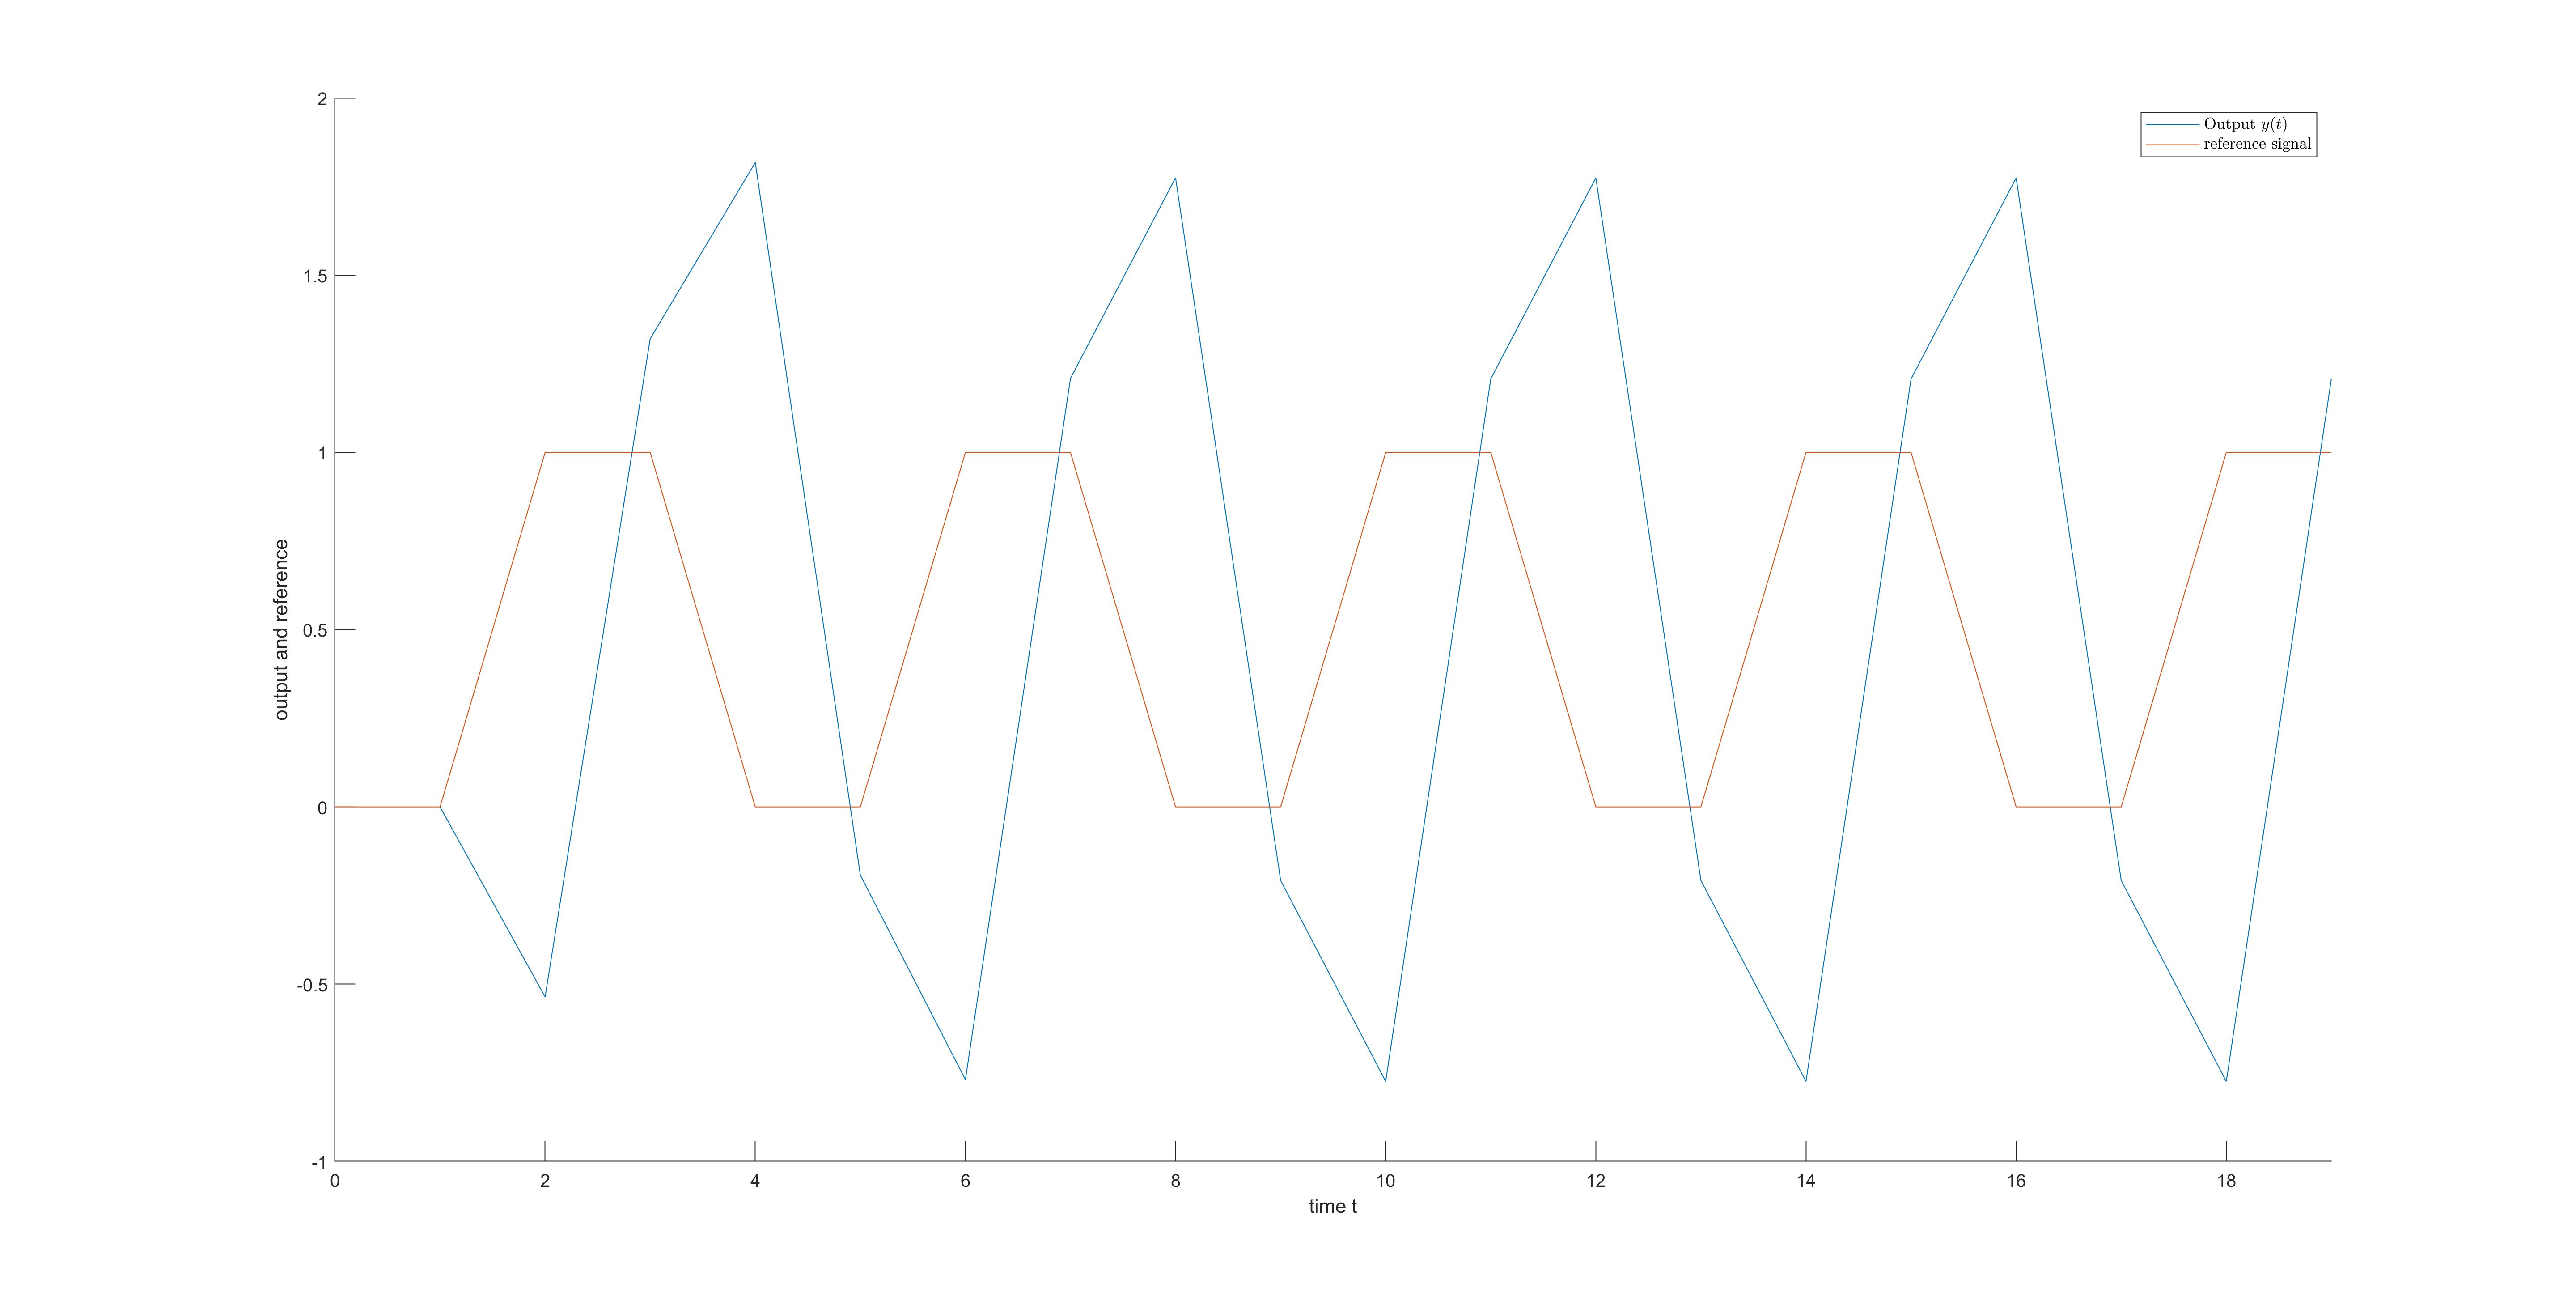
\includegraphics[width=\textwidth]{fig/LQR_ex.jpg}
	\caption{Tracking with controller based on separation principle for system \eqref{eq:ILC:Sys_ex1}}
\end{figure}
\end{example}



As one can see, the tracking in Example \ref{ex:ILC:LQR} is not perfect at all. However, we can extract a bunch of information from this controlled system. For example, we get the input and output sequences 
\begin{align}
&\{u(0), \, u(1), \,  u(2) \, \dots , \, u(N)\} \subset \R^l \label{eq:ILC:u_seq} \\
&\{y(0), \, y(1), \, y(2) , \, \dots , \, y(N)\}\subset \R^m.\label{eq:ILC:y_seq}
\end{align}
This sequences are limited due to the finite time horizon. It seems to be an advantage. 

Indeed, if we put the signals we got from simulation together, we get a big, but finite dimensional vector. That means, the standard tools from linear algebra can be applied. 

As a matter of fact, we can express our whole simulated system as a linear equation. We call such vectors \textit{Supervectors}, and the whole system is said to be ''lifted''.

\section{Supervector description} 

For the sequences \eqref{eq:ILC:u_seq} and \eqref{eq:ILC:y_seq} we define the supervectors
\begin{align}
\label{eq:inoutsuper}
u = \begin{pmatrix}
u(0) \\ u(1) \\ u(2) \\ \vdots \\ u(N)
\end{pmatrix} \in \R^{l(N+1)}, \;
y = \begin{pmatrix}
y(0) \\ y(1) \\ y(2) \\ \vdots \\ y(N)
\end{pmatrix} \in \R^{m(N+1)}.
\end{align}

Respectively, we determine supervectors $r\in \R^{m(N+1)}$ and $e\in \R^{m(N+1)}$. 

For system \eqref{eq:GP} the relation between $u$ and $y$, and the error $e$ can be written in a linear matrix form 
\begin{align}
\label{eq:Gu + d}
y &= Gu + d, \\
e &= r - y.
\end{align}
The matrix $G$ represents here the state-space model and is given via  
\begin{align}
\label{eq:Gmatrix}
\begin{split}
G &= G(A,B,C,D) = \\
&=  \begin{pmatrix}
D & 0 & \cdots & 0 & 0 & 0 \\
CB & D & \cdots & 0 & 0 & 0\\
CAB & CB & \cdots & 0 & 0 & 0\\
\vdots & \vdots & \ddots & \vdots  & \vdots & \vdots \\
CA^{N-2} B & CA^{N-3} B &\dots &CB & D& 0\\
CA^{N-1} B & CA^{N-2} B &\dots &CAB & CB& D\\
\end{pmatrix} \in \R^{m(N+1)\times l(N+1)}.
\end{split}
\end{align}
The vector $d$ depends on the initial condition $x_0$:
\begin{align}
d = d(C,A,x_0) = \begin{pmatrix}
C x_0 \\ CA x_0 \\ CA^2 x_0 \\ \vdots \\ CA^Nx_0
\end{pmatrix} \in \R^{m(N+1)}.
\end{align}


It looks pretty simple! 

If we know the signal $r$ we want to track, we can find a perfect solution by choosing 
\begin{align}
u_\infty = G^{-1} r -d.
\end{align}

However, this choice does not look greatly  credible. 

For example, if our system is uncertain and is described by $\t G$, but modeled by $G$, we get 
\begin{align}
e = r - y = (I - \t G G^{-1} ) r. 
\end{align}

This error might be non-zero, even for a little model perturbations. 
Besides, the matrix $G$ might be singular and do not have an inverse. 

Still it can have a right or left inverse. 
If we can reformulate this idea in a more robust way, we may get a good and simple applicable algorithm, which we call the inverse model algorithm.

\section{Inverse Model Algorithms}

\begin{alg}
	\label{alg: rightInv}
	Let the matrix $D$ in \eqref{eq:GP} have full row rank. Then the matrix $G = G(A, B, C, D)$ has a right inverse $G_R$: 
	\begin{align*}
	G G_R = I. 
	\end{align*}
	The Right Inverse Model Algorithm (RIA) is given via input update law 
	\begin{align}
	\label{eq:errRightInv}
	\begin{split}
	u_{k+1} &= u_k + \beta G_R e_k, \\
	u_0& \in \R^{l (N+1)},
	\end{split}	
	\end{align}
	with error evolution
	\begin{align}
	\label{eq:Alg:e_k+1 = (1 - beta) e_k}
	\begin{split}
	e_{k+1} &= (1- \beta) e_{k}, \; k\geq 0, \\
	e_0 &= r -  Gu_0 -d.
	\end{split}
	\end{align}
	In particular, $(e_k)_{k\geq 0}$ converges to zero for $k \to \infty$ for any initial error $e_0 \in \R^{m(N+1)}$ if and only if 
	\begin{align*}
	0 < \beta < 2.
	\end{align*}
\end{alg}
\begin{proof}
	Firstly, the matrix $G$ has lower triangular structure, with the matrix $D$ on its diagonal. Hence, $G$ has full row rank if and only if $D$ has the full row rank.
	Taking the limit over relation \eqref{eq:Alg:e_k+1 = (1 - beta) e_k} results in
	\begin{align}
	\lim_{k \to \infty} e_{k+1} = \lim_{k \to \infty}(1- \beta) e_{k} = \lim_{k \to \infty}(1 - \beta)^k e_0.
	\end{align}
	
	Choosing $0<\beta < 2$ yields the proof. 
\end{proof}

For $\beta$ close to 0 or 2, we get slower convergence and better robustness. For $\beta = 1$ we get convergence in one iteration, but this choice might be highly non-robust \cite{ILC}, pp 149, 152-155.

If there exists (only) a left inverse of $G$, we can also calculate a better choice of input $u$. But in this algorithm, we do not have a guarantee of zero-convergence. 


\begin{alg}
	\label{alg: leftInv}
	Let the matrix $D$ in \eqref{eq:GP} have full column rank. Then the matrix $G = G(A, B, C, D)$ has a left inverse $G_L$: 
	\begin{align*}
	G_L G = I. 
	\end{align*}
	The Left Inverse Model Algorithm (LIA) is given via input update law
	\begin{align}
	\begin{split}
	u_{k+1} &= u_k + \beta G_L e_k, \; k\geq 0 \\
	u_0& \in \R^{l (N+1)}. 
	\end{split}	
	\end{align}
	with error evolution
	\begin{align}
	\label{eq:errLeftInv}
	\begin{split}
	e_{k} &= (I- \beta G G_L) e_{k-1} = (I+  \left[(1-\beta)^{k-1} - 1\right] G G_L) e_0, \; k\geq 1, \\
	e_0 &= r -  Gu_0 -d.
	\end{split}
	\end{align}
	Monotonic convergence to 
	\begin{align}
	\label{eq:leftInvErrLim} 
	e_\infty  = \lim_{k\to\infty} e_k = (I - G G_L)e_0
	\end{align} 
	for $k \to \infty$ is guaranteed if and only if 
	\begin{align*}
	0 <\beta < 2.
	\end{align*}
\end{alg}
\begin{proof}
	Firstly, the matrix $G$ has lower triangular structure, with the matrix $D$ on its diagonal. Hence, $G$ has full column rank if and only if $D$ has the full column rank.
	
	Using the relation $(GG_L)^2 = GG_LGG_L = GG_L$ the error evolution formula \eqref{eq:errLeftInv} can be proven by mathematical induction: 
	
	for $k = 1$ it follows: 
	\begin{align*}
	e_1 = (I - \beta G G_L)e_0 = (I + GG_L - GG_L - \beta G G_L)e_0 = (I + \left[(1 - \beta) + 1\right]GG_L)e_0.
	\end{align*}
	
	For $k \in \N$  
	\begin{align*}
	e_{k+1} &= ( I - \beta G G_L)e_k = ( I - \beta G G_L) (I+  \left[(1-\beta)^{k-1} - 1\right] G G_L) e_0 = \\
	& = \left(I - \beta G G_L + (1-\beta)^{k-1}GG_L - GG_L - \beta GG_L\left[(1 - \beta)^{k-1} - 1\right]GG_L\right)e_0=\\
	& = \left(I - (\beta - (1-\beta)^{k-1} + \beta\left[(1 - \beta)^{k-1} - 1\right])G G_L\right)e_0\\
	& = \left(I - \left(\beta - (1-\beta)^{k-1} + 1 + \beta(1-\beta)^{k-1} - \beta\right)GG_L\right)e_0\\
	& = (I+  \left[(1-\beta)^k - 1\right] G G_L) e_0
	\end{align*}
	
	To prove \eqref{eq:leftInvErrLim} recall that 
	\begin{align*}
	\R^{m(N+1)} = \im(G)\oplus \ker (G_L). 
	\end{align*}
	Hence $e_0$ can be written as 
	\begin{align*}
	e_0 = G w_0 + v_0,
	\end{align*}
	where $v_0 = (I - G G_L)e_0 \in \ker (G_L)$  is uniquely defined and $w_0 = G_L e_0 \in \R^{l(N+1)}$. It follows: 
	\begin{align*}
	e_{k} = (1+ \left[(1 - \beta)^{k-1} - 1\right]GG_L)e_0 = (1-\beta)^{k-1} G w_0 + v_0.
	\end{align*}
	Then for $\beta \in (0,2)$ the error $e_k$ converges to $v_0$ for $k \to \infty$. 
\end{proof} 



The choice of $\beta$ is identical to this in Algorithm \ref{alg: rightInv}.

\begin{exam}
	For the system \eqref{eq:ILC:Sys_ex1} we can apply the Right Inverse Mode Algorithm. 
	
	Result for $N = 20$ and $\beta = .1$ is illustrated in Figure  
	
	\begin{figure}[ht]
		\label{img:ILC:RIA}
		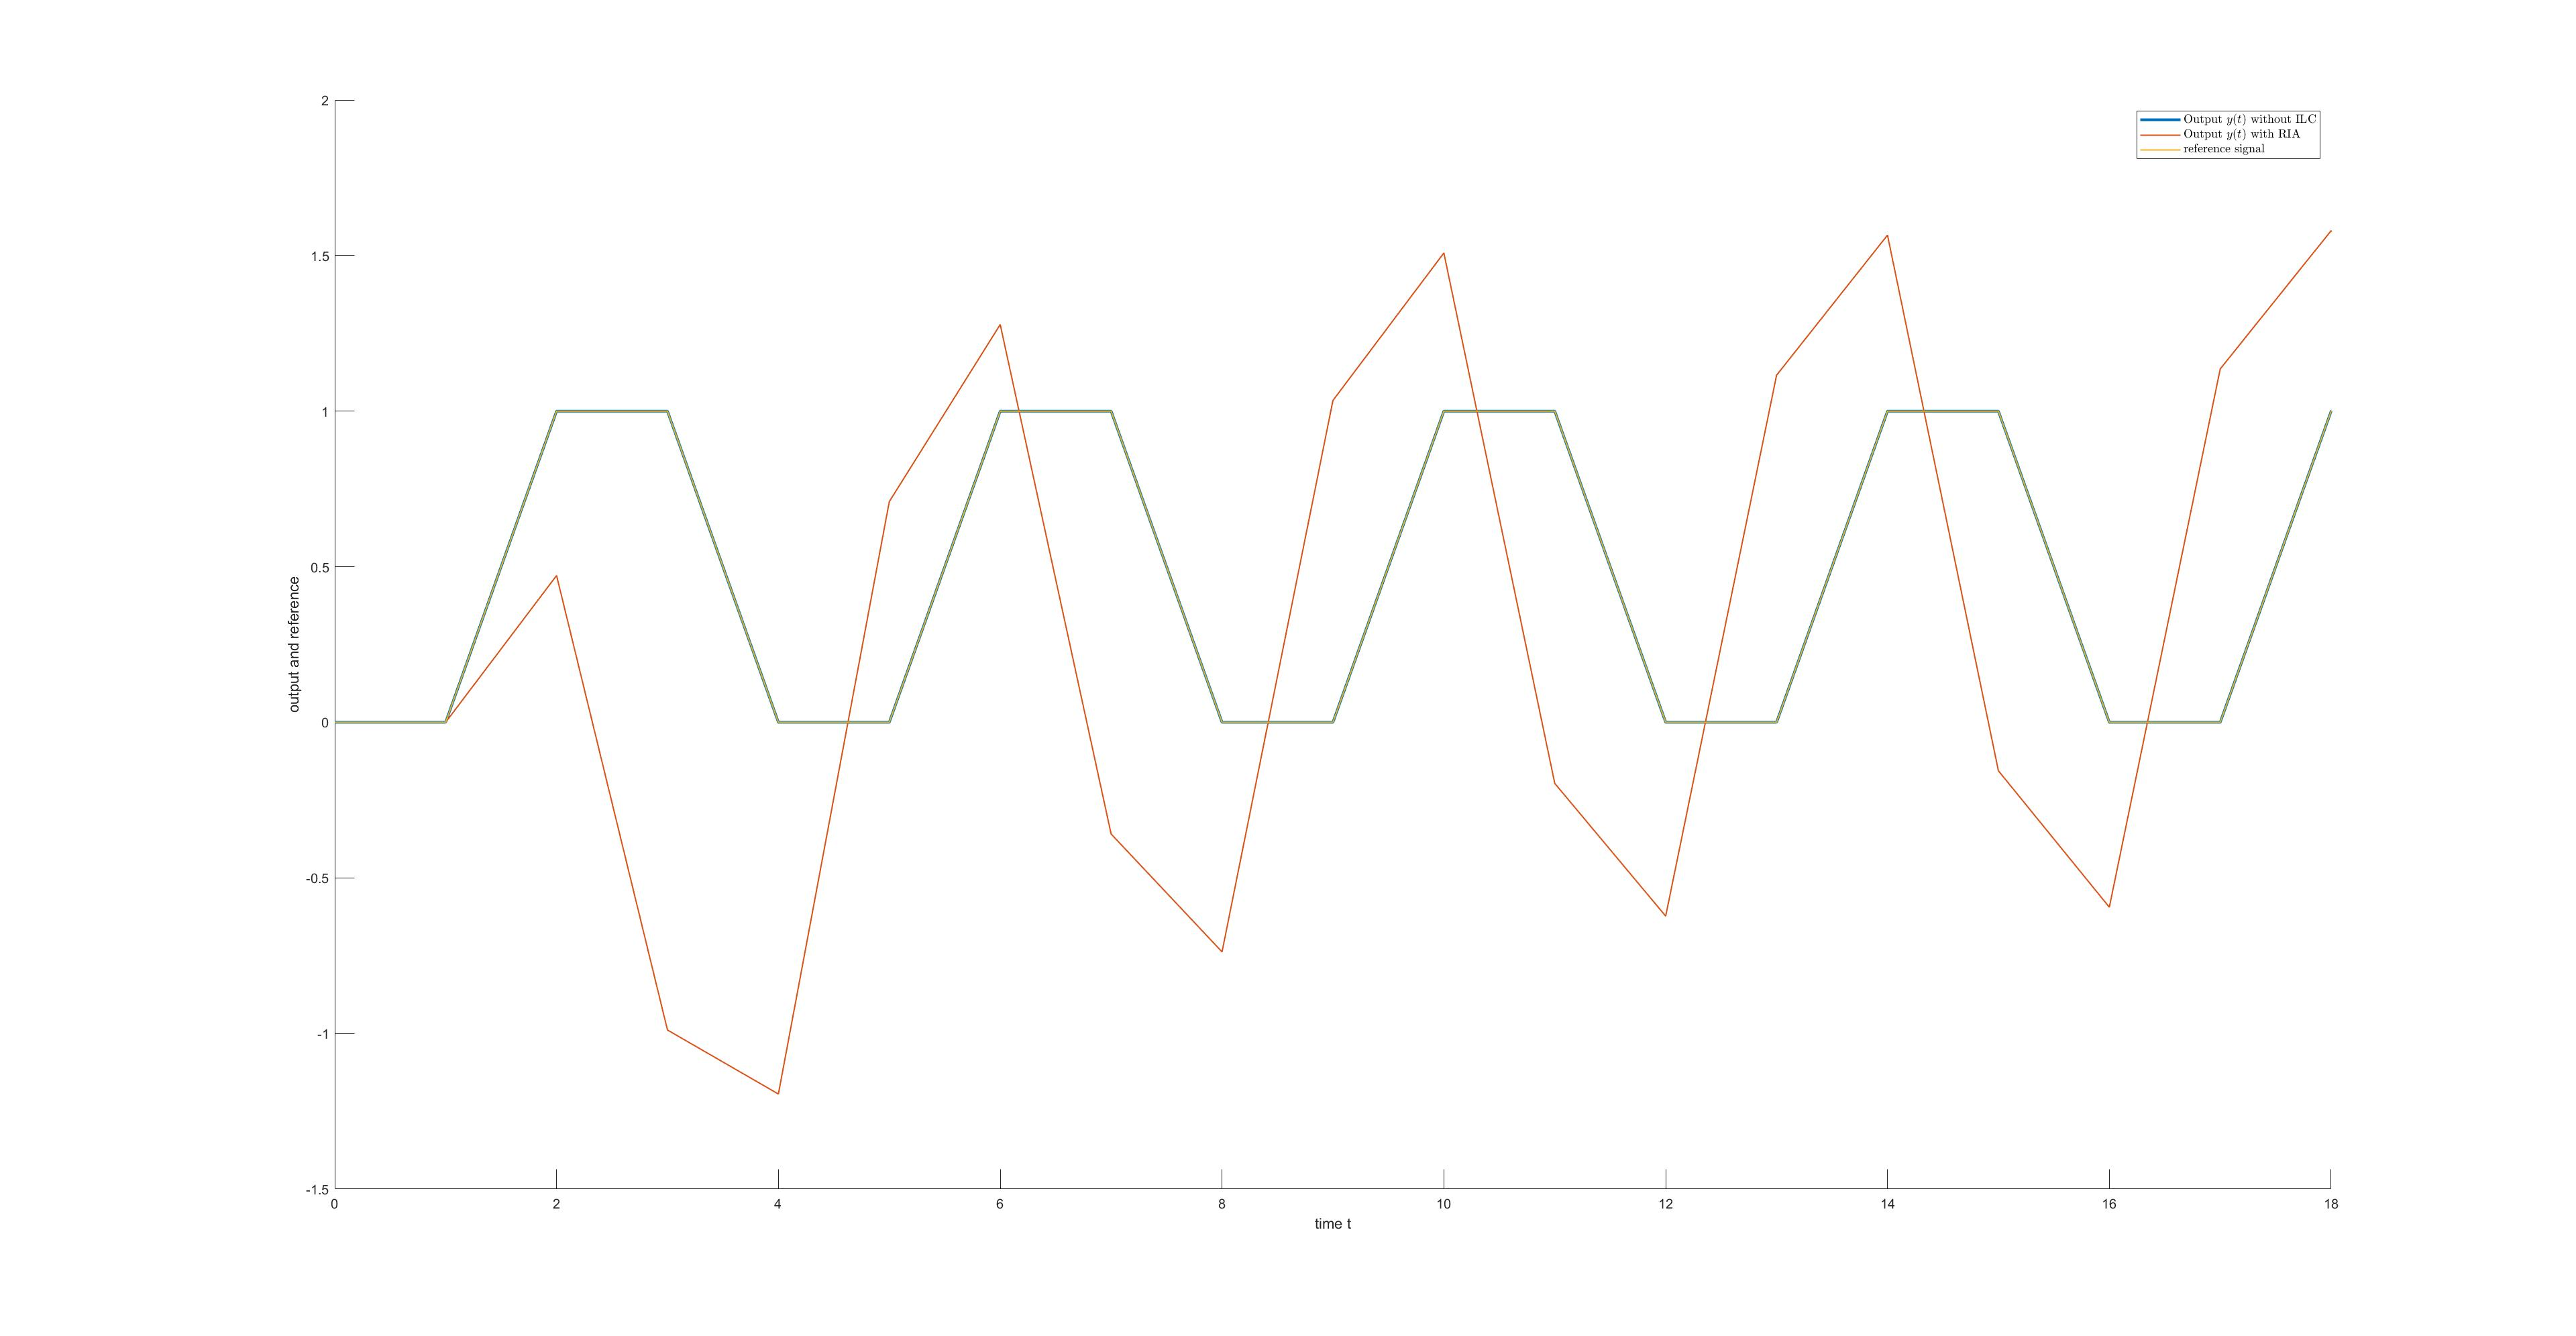
\includegraphics[width=\textwidth]{fig/RIA.jpg}
		\caption{Tracking with LQR Controller (without ILC Algorithm), and tracking with Right Inverse Model Algorithm for the system \eqref{eq:ILC:Sys_ex1}}, with pulse reference signal (RIA UND LQR SIND VERTAUSCHT!!!!) %TODO
	\end{figure}
	
	
\end{exam}

Right and Left Inverse Model Algorithms belong to the class of so-called Unit Memory Algorithms. 

Indeed, we can formulate such algorithms more general. 

\section{Unit Memory Algorithm}

We are interested in  the processes, which are executed repetitively. Let $k = 0, \, 1, \, 2, \, \dots $ be the number of completed iterations. Then we get a system 
\begin{align}
\label{eq:unitMemory}
\begin{split}
y_{k} &= G u_k + d,  \\ %& &\text{ (The Input Update Rule)} 
e_k &= r - y_k, 
\end{split}
\end{align}
$u_{0} \in \R^{l(N+1)},  \; k =0, \,  1, \, 2, \dots $ .
This is again a discrete-time system, with time increment $k$. 

To achieve a good tracking we need to ensure the norm $||e_k||$ to be small for large $k$. 
A better tracking can be achieved, if the convergence is monotone, i.e. 
\begin{align}
||e_{k+1} || < ||e_k|| \text{ for all } k \geq 0.
\end{align}

The asymptotically perfect tracking means
\begin{align}
\lim_{k\to\infty} ||e_k|| = 0.
\end{align}

We have already seen, that it is not always possible to achieve zero convergence. In Algorithm \ref{alg: leftInv} the perfect tracking is possible, if the reference signal $r$ is feasible. In common the convergence properties can also depend on the choice $u_0$.

%the monotonic convergence to some $e_\infty \in \R^{m(N+1)}$ is desirable :
%\begin{align}
%\lim_{k \to \infty} e_k = e_\infty, \text{ and } ||e_{k+1} || \leq ||e_k|| \text{ for all } k \geq 0.
%\end{align}

%First we try to formulate an iteration law for the input signal, and calculate then the error sequence as 
%\begin{align}
%e_k = r - y_k = r - G u_k - d, k \geq 0.
%\end{align}

We assume linear dependency of $u_{k+1}$ upon $u_k$ and $e_k$ for $k \geq 0$, and define the following algorithm using feedback control. 
\begin{alg}
	\label{alg: unitMemory}
	The Unit Memory Algorithm is given via input update law 
	\begin{align}
	\label{eq:clPlant}
	\begin{split}
	u_{k+1} &= u_k + K e_k, \\
	& u_0 \in \R^{l (N+1)}.
	\end{split}
	\end{align}	 
	The error dynamic is then given via
	\begin{align}
	e _{k+1} &= (I - G K) e_{k}, \; k \geq 0,\\
	e_0 &= r -  Gu_0 -d.
	\end{align}
%	since 
%	\begin{align}
%	\begin{split}
%	e_{k+1} &=  r - y_{k+1} = r - G u_{k+1} - d =\\
%	&= r - Gu_k - G Ke_k - d = e_k - G Ke_k, \; k\geq0.
%	\end{split}
%	\end{align}
	$K \in \R^{l(N+1) \times m(N+1)}$ is called \textbf{learning matrix}. 
\end{alg}

To ensure the stability of the algorithm, it is enough to consider the iteration process 
\begin{align}
\label{eq:e_k}
e_{k+1} = (I - G K) e_k = (I - G K)^k e_0  : =  L^k e_{0}, \; k \geq 0.
\end{align}

That it is a discrete dynamical system over $k$. We can reformulate our goal as follows: find some matrix $K \in \R^{l(N+1) \times m (N+1)}$, which renders \eqref{eq:e_k} stable. %In other words, we are looking for a stabilizing controller $K$. 

We can also rewrite our system as
\begin{align}
\label{eq:ILC:e_kPlant}
\begin{pmatrix}
e_{k+1} \\ e_k
\end{pmatrix} = 
\left(
\begin{array}{c|c}
I & -G \\\hline K & 0
\end{array}\right) \begin{pmatrix}
e_k \\ v_k 
\end{pmatrix}
\end{align}

Then our problem is reduced to finding a stabilizing controller $K$  with 
\begin{align}
v_k = K e_k.
\end{align} 

We know how to work with such systems -- for example, LQR controller provides a good solution. This is a reliable method, but since the matrix $G$ can be large, it also can be too costly. Often we can achieve good results with much more simple methods. For example, we can reduce the number of parameters to be chosen. 

In the Algorithms \ref{alg: rightInv} and \ref{alg: leftInv}: we choose the fixed matrix $K_0$ and as right or left inverse of the matrix $G$, and leave the parameter $\beta$ to decide on. 

However, these algorithms have a big disadvantage: the numerical calculation might be inaccurate even for right and left inverse, -- or quite impossible if the matrix $G$ does not have full row/column rank. We illustrate it in the following example. 

\begin{exam}
	\label{ex:ILC:IAcrushes}
	We consider again our system \eqref{eq:ILC:Sys_ex1}. 
	
	We have seen, that for $N = 20$ we can achieve good and robust results. 
	But how does it look for larger $N$? 
	
	Let us consider the case $N = 40$. 
	The error evolution does not depend on the inverse model, and hence converges as expected to 0 (Figure \ref{fig:ILC:IA_N40}). 
	
	But once we try to apply calculated result to our system, we do not see good tracking (Figure \ref{fig:ILC:IA_N_output40}). Quite the same we get a large discrepancy between the reference signal and the system output. 
	
	If we write our error evolution as 
	\begin{align}
	\label{eq:ILC:ex_IA1}
	e_k = r - Gu_k - d, \text{ for } k \geq 0, \tag{*}
	\end{align}
	we can observe a quite different picture compared to the error evolution 
	\begin{align}
	\label{eq:ILC:ex_IA2}
	e_k = (1 - \beta)^k e_0,\; k\geq 0. \tag{**}
	\end{align}
	We illustrate it in the Figure \ref{fig:ILC:A}. 
	
	The reason might be the condition number of the matrix $G$, which equals 1.0137e+18. 
	
	
	\begin{figure}[ht!]
		\centering
		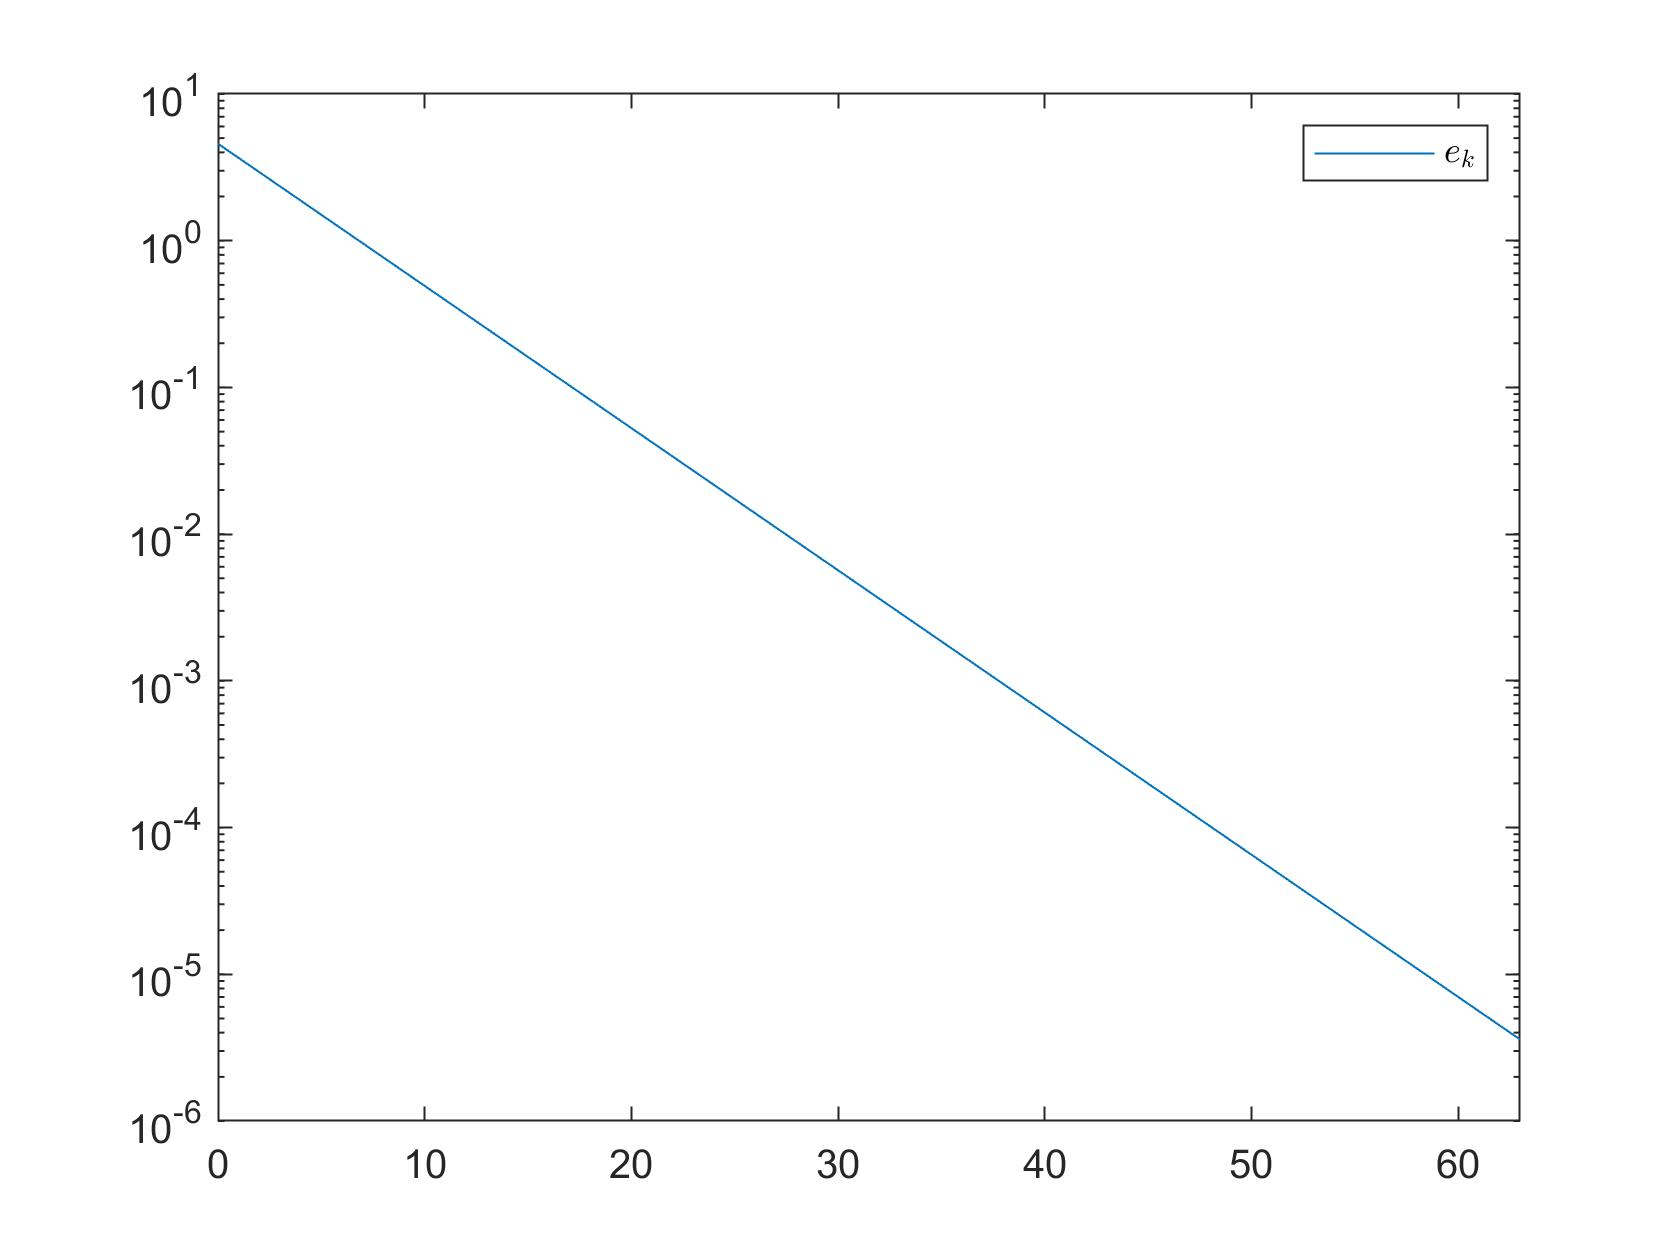
\includegraphics[width=\textwidth]{fig/IA_N40.jpg}
		\caption{Error evolution calculated with \eqref{eq:ILC:ex_IA1} in Right Inverse Model Algorithm for \ref{ex:ILC:IAvsSDA}}
		\label{fig:ILC:IA_N40}
	\end{figure}
	
	\begin{figure}[ht!]
		\centering
		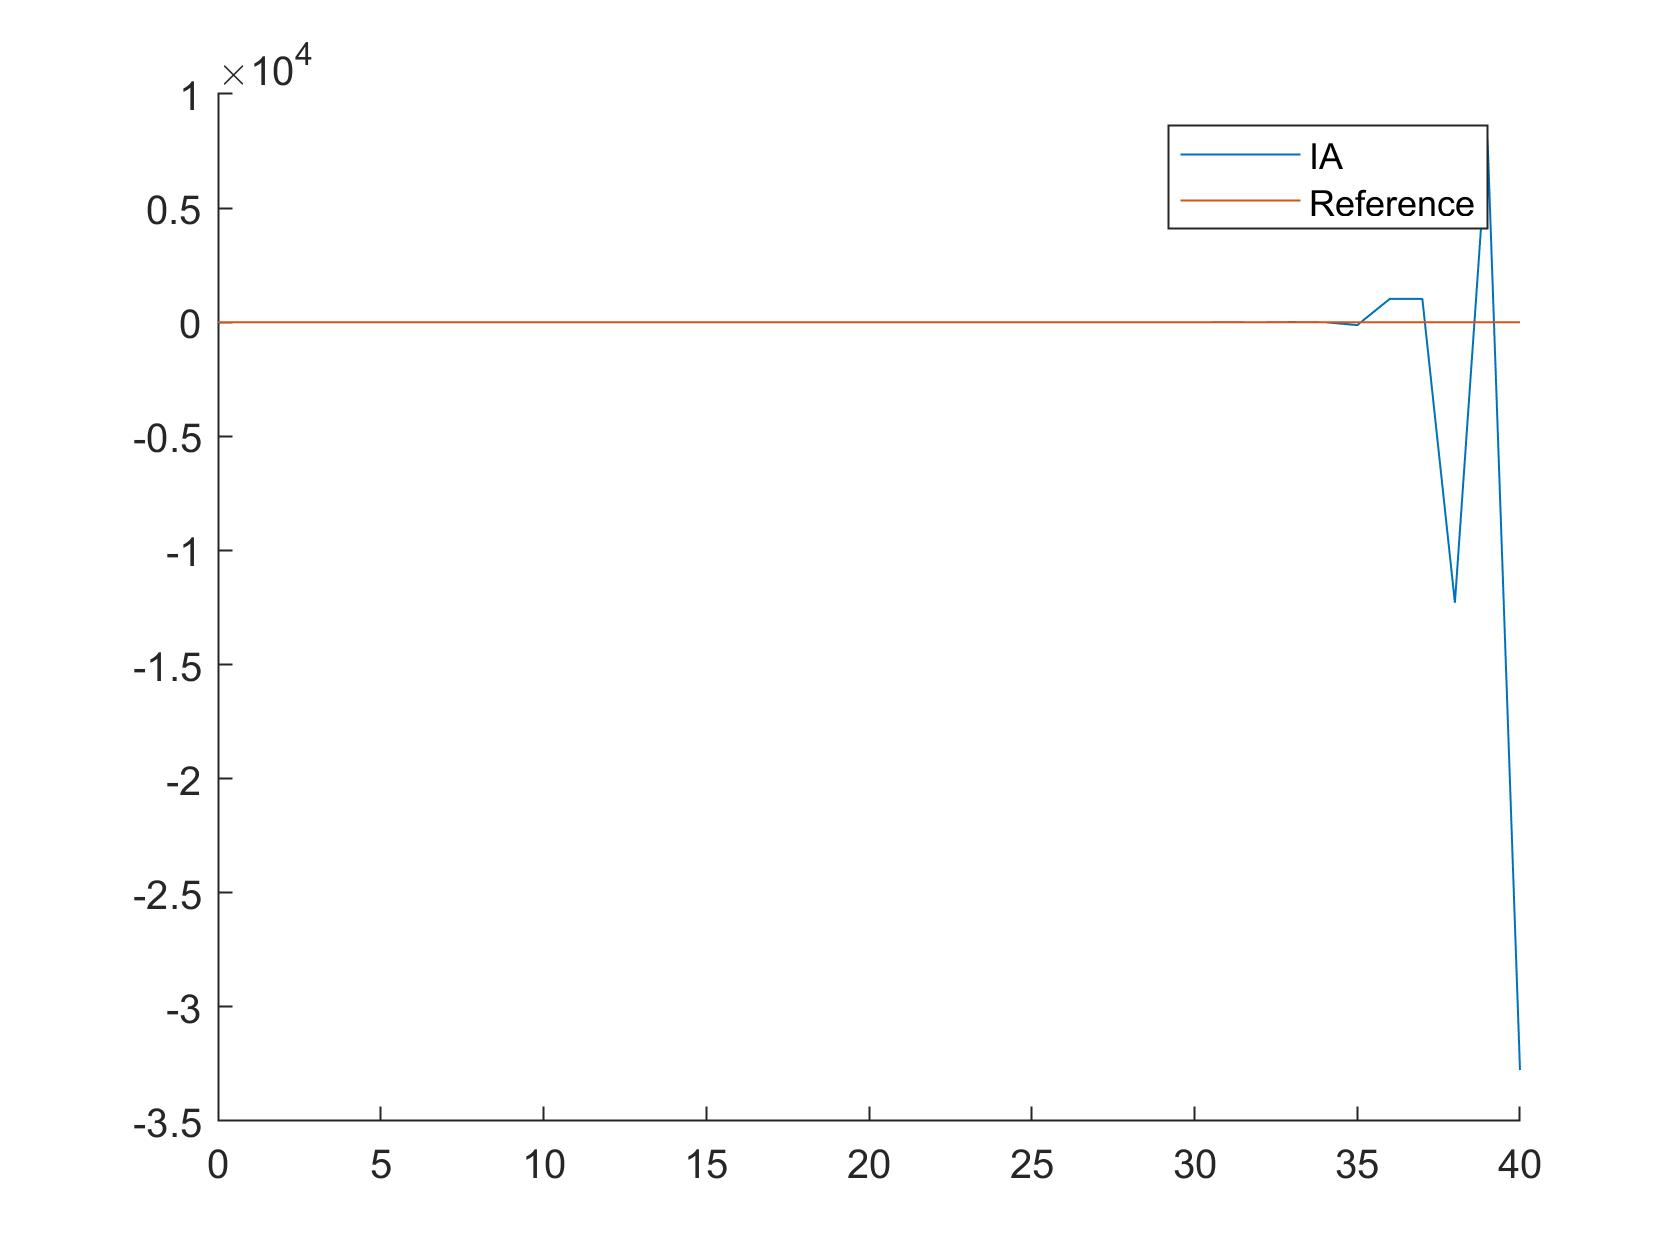
\includegraphics[width=\textwidth]{fig/IA_N40_output.jpg}
		\caption{Application of the result of RIA for \ref{eq:ILC:Sys_ex1} for $N = 40$}
		\label{fig:ILC:IA_N_output40}
	\end{figure}
	
	
	\begin{figure}[ht!]
		\centering
		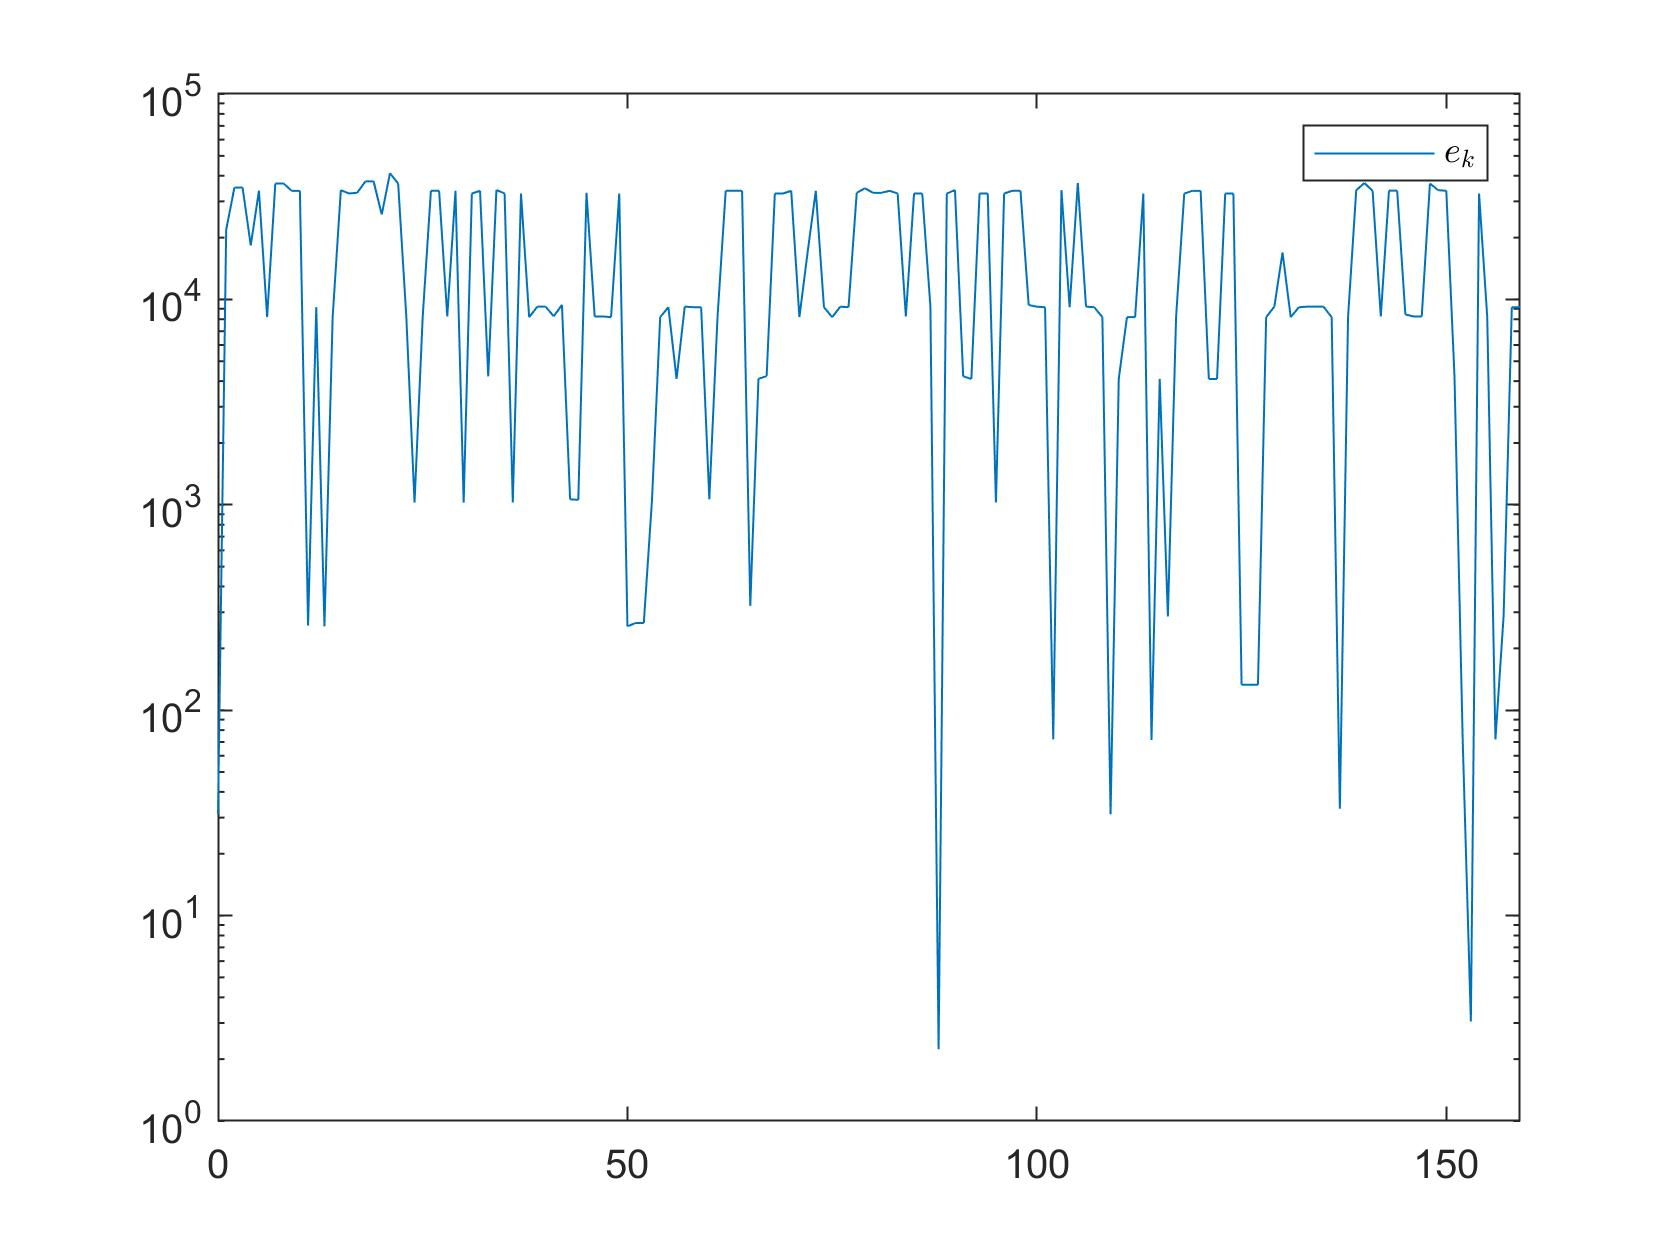
\includegraphics[width=\textwidth]{fig/IA_N40_errorEv2.jpg}
		\caption{Error evolution calculated with \eqref{eq:ILC:ex_IA2} in Right Inverse Model Algorithm for \ref{eq:ILC:Sys_ex1}}
			\label{fig:ILC:A}
	\end{figure}
	
\end{exam}


An algorithm, which does not require the model inversion, might be here of use. 

%This leads to plain but essential result: 
%
%\begin{theo}
%	\label{thm: rho(L)<1}
%	\begin{enumerate}
%		\item The closed-loop \ref{eq:clPlant} is stable if and only if the matrix $L$ satisfies 
%		\begin{align}
%		\rho(L) < 1,
%		\end{align}
%		\item If $\rho(L) = 1$, then $\lim_{k \to \infty} L^k = \hat{L}$ for some $\hat{L}\in \R^{m(N+1)\times m(N+1)}$ and the sequence $(e_k)_{k\geq 0}$ is monotonically decreasing and converges to $e_\infty = \hat{L}e_0$, if and only if for $L$ all Jordan Blocks of the eigenvalue 1  have dimension 1. If in additional $e_0 \in \ker(\hat{L})$, then monotone convergence to 0 is guaranteed. 
%	\end{enumerate}
%\end{theo} 
%
%\begin{proof}
%	%TODO: Proof zuende schreiben 
%	{\color{red} Hier wird es proof geben} 
%	%The proof of both statements is based on using of Jordan Normal Form. 
%	%Let $L$ have the eigenvalues $\lambda_1, \lambda_2, \dots , \lambda_{l_N+1}$ with multiplicity $n_1, n_2, \dots , n_{l(N+1)}$. 
%	%There exists a non-singular matrix $T$, such that 
%	%\begin{align}
%	%L = T J T^{-1}, \; J = \diag(J_1, J_2, \dots , J_p),
%	%\end{align}
%	%where $J_i$ represents a $i$-th Jordan Block, $ i = 1, 2, \dots , q$. 
%	%Then $L^k = T J^k T^{-1}$, and $J^k = diag(J_1^k, J_2^k, \dots , J_q^k)$, each Jordan Block has the form 
%	%\begin{align}
%	%J_j = 
%	%\begin{pmatrix}
%	%\lambda_j & 1 & 0 & \cdots & 0 & 0\\
%	%0 & \lambda_j & 1 & \cdots & 0 & 0 \\
%	%\vdots & \vdots & \ddots & \ddots & \vdots & \vdots &\\
%	%0 & 0 & 0 & \cdots & \lambda_j & 1\\
%	%0 & 0 & 0 & \cdots & 0 & \lambda_j \\
%	%\end{pmatrix}
%	%\end{align}
%	
%\end{proof}
%
%We will see, that it is often not possible, to achieve $\rho(L) < 1$. Still, the convergence to 0 is attainable. Since $e_0$ depends on $u_0$ and $r$, the design problem here is to find adequate target $r$ -- usually that means, that it must be feasible -- and a good start input value $u_0$. Furthermore, the matrix $K$ is still a design issue in Unit Memory Algorithm, since it allows us to regulate the spectrum of $L$. 
%
%\section{Inverse Model Algorithm}
%
%Let us come back to the original problem \eqref{eq:Gu + d}. 
%If the matrix $G$ is invertible, the choice $K = G^{-1}$ leads to 
%\begin{align*}
%e_{k+1} = (I - G G^{-1})e_k = 0 \text{ for all } k \geq 0,
%\end{align*}
%and the resulting input signal for ''perfect tracking'' is given after a single iteration by 
%\begin{align*}
%u_\infty = G^{-1}(r-d). 
%\end{align*}
%
%This looks pretty simple, so why do we still need some iteration algorithms? 
%Firstly, the matrix $G$ might not have an inverse. Though we can still find the precise solution if the right inverse $G_R$ exists. But if there exists only a left inverse $G_L$ we get $e_{k+1} = (I - G G_L)e_k$ which might be non zero. 
%Secondary, if the model is inaccurate, this solution might differ significantly from the true one \cite{ILC}.
%
%A more plausible design is to choose $K = \beta \hat{G}$ for some real constant $\beta$, where $\hat{G}$ is the left or right inverse of $G$. This allows a trade-off between the robustness and the convergence rate. 
%
%\begin{alg}
%	\label{alg: rightInv}
%	Let the matrix $D$ in \eqref{eq:GP} have full row rank. Then the matrix $G = G(A, B, C, D)$ has a right inverse $G_R$: 
%	\begin{align*}
%	G G_R = I. 
%	\end{align*}
%	The Right Inverse Model Algorithm is characterized by choosing  $K = \beta G_R$, where $\beta$ is a real scalar, called ''learning gain''.
%	Then input update law is given via 
%	\begin{align}
%	\label{eq:errRightInv}
%	\begin{split}
%	u_{k+1} &= u_k + \beta G_R e_k, \\
%	u_0& \in \R^{l (N+1)},
%	\end{split}	
%	\end{align}
%	with error evolution
%	\begin{align}
%	\label{eq:Alg:e_k+1 = (1 - beta) e_k}
%	\begin{split}
%	e_{k+1} &= (1- \beta) e_{k}, \; k\geq 0, \\
%	e_0 &= r -  Gu_0 -d.
%	\end{split}
%	\end{align}
%	In particular, $(e_k)_{k\geq 0}$ converges to zero for $k \to \infty$ for any initial error $e_0 \in \R^{m(N+1)}$ if and only if 
%	\begin{align*}
%	0 < \beta < 2.
%	\end{align*}
%\end{alg}
%\begin{proof}
%	Firstly, the matrix $G$ has lower triangular structure, with the matrix $D$ on its diagonal. Hence, $G$ has full row rank if and only if $D$ has the full row rank.
%    Taking the limit over relation \eqref{eq:Alg:e_k+1 = (1 - beta) e_k} results in
%    \begin{align}
%	\lim_{k \to \infty} e_{k+1} = \lim_{k \to \infty}(1- \beta) e_{k} = \lim_{k \to \infty}(1 - \beta)^k e_0.
%    \end{align}
%    
%    Choosing $0<\beta < 2$ yields the proof. 
%\end{proof}
%
% For $\beta$ close to 0 or 2, we get slower convergence and better robustness. For $\beta = 1$ we get convergence in one iteration, but this choice might be highly non-robust \cite{ILC}, pp 149, 152-155.
%
%If there exists (only) a left inverse of $G$, we can also calculate a better choice of input $u$. But in this algorithm, we do not have a guarantee of zero-convergence. 
%
%
%\begin{alg}
%	\label{alg: leftInv}
%	Let the matrix $D$ in \eqref{eq:GP} have full column rank. Then the matrix $G = G(A, B, C, D)$ has a left inverse $G_L$: 
%	\begin{align*}
%	G_L G = I. 
%	\end{align*}
%	The Left Inverse Model Algorithm is characterized by choosing $K = \beta G_L$, where $\beta$ is a real scalar, called ''learning gain''. The  input update law has the form
%	\begin{align}
%	\begin{split}
%	u_{k+1} &= u_k + \beta G_L e_k, \; k\geq 0 \\
%    u_0& \in \R^{l (N+1)}. 
%	\end{split}	
%	\end{align}
%	with error evolution
%	\begin{align}
%	\label{eq:errLeftInv}
%	\begin{split}
%		e_{k} &= (I- \beta G G_L) e_{k-1} = (I+  \left[(1-\beta)^{k-1} - 1\right] G G_L) e_0, \; k\geq 1, \\
%		e_0 &= r -  Gu_0 -d.
%	\end{split}
%	\end{align}
%	Monotonic convergence to 
%	\begin{align}
%	\label{eq:leftInvErrLim} 
%	e_\infty  = \lim_{k\to\infty} e_k = (I - G G_L)e_0
%	\end{align} 
%	for $k \to \infty$ is guaranteed if and only if 
%	\begin{align*}
%	0 <\beta < 2.
%	\end{align*}
%\end{alg}
%\begin{proof}
%	Firstly, the matrix $G$ has lower triangular structure, with the matrix $D$ on its diagonal. Hence, $G$ has full column rank if and only if $D$ has the full column rank.
%	
%	Using the relation $(GG_L)^2 = GG_LGG_L = GG_L$ the error evolution formula \eqref{eq:errLeftInv} can be proven by mathematical induction: 
%	
%	for $k = 1$ it follows: 
%	\begin{align*}
%	e_1 = (I - \beta G G_L)e_0 = (I + GG_L - GG_L - \beta G G_L)e_0 = (I + \left[(1 - \beta) + 1\right]GG_L)e_0.
%	\end{align*}
%	
%	For $k \in \N$  
%	\begin{align*}
%	e_{k+1} &= ( I - \beta G G_L)e_k = ( I - \beta G G_L) (I+  \left[(1-\beta)^{k-1} - 1\right] G G_L) e_0 = \\
%	& = \left(I - \beta G G_L + (1-\beta)^{k-1}GG_L - GG_L - \beta GG_L\left[(1 - \beta)^{k-1} - 1\right]GG_L\right)e_0=\\
%	& = \left(I - (\beta - (1-\beta)^{k-1} + \beta\left[(1 - \beta)^{k-1} - 1\right])G G_L\right)e_0\\
%	& = \left(I - \left(\beta - (1-\beta)^{k-1} + 1 + \beta(1-\beta)^{k-1} - \beta\right)GG_L\right)e_0\\
%	& = (I+  \left[(1-\beta)^k - 1\right] G G_L) e_0
%	\end{align*}
%	
%	To prove \eqref{eq:leftInvErrLim} recall that 
%	\begin{align*}
%	\R^{m(N+1)} = \im(G)\oplus \ker (G_L). 
%	\end{align*}
%	Hence $e_0$ can be written as 
%	\begin{align*}
%	e_0 = G w_0 + v_0,
%	\end{align*}
%	where $v_0 = (I - G G_L)e_0 \in \ker (G_L)$  is uniquely defined and $w_0 = G_L e_0 \in \R^{l(N+1)}$. It follows: 
%	\begin{align*}
%	e_{k} = (1+ \left[(1 - \beta)^{k-1} - 1\right]GG_L)e_0 = (1-\beta)^{k-1} G w_0 + v_0.
%	\end{align*}
%	Then for $\beta \in (0,2)$ the error $e_k$ converges to $v_0$ for $k \to \infty$. 
%\end{proof} 
%
%
%
%The choice of $\beta$ is identical to this in Algorithm \ref{alg: rightInv}.

\section{Gradient Algorithms}
We can begin to define a new algorithm with the requirements on it. We want this algorithm to be monotonic convergent, so we can easily decide on termination criterion. 

The direct calculation provides 
\begin{align}
\label{eq:monConv}
||e_{k+1}|| < ||e_k|| \text{ for all } k >0,
\end{align}

in some norm $|| \cdot || $ in $\R^{m(N+1)}$. 

We chose some positive definite weighting matrices $Q(t)$ and $R(t)$, $t = 0, 1, 2, \dots ,N$, and define the scalar products
\begin{align}
\label{eq:SkPrQR}
\langle y,z\rangle_Q = \sum_{t = 0}^N y(t)^TQ(t)z(t), \; \langle u,v\rangle_R = \sum_{t = 0}^N u(t)^T R(t) v(t).
\end{align}

We denote with $||\cdot||_Q$ and $||\cdot||_R$ the associated norms, and set
\begin{align*}
G^\star &= R^{-1} G^T Q \text{ for all } G \in \R^{m(N+1)\times l(N+1)},\\
K^\star &= Q^{-1} K^T R \text{ for all } K \in \R^{l(N+1)\times m(N+1)},
\end{align*}
where 
\begin{align}
Q := \diag(Q(0), Q(1), Q(2) ,\dots, Q(N)) \text{ and } R:= \diag(R(0), R(1), R(2), \dots, R(N)).
\end{align}
In the same way, we can define 
\begin{align}
L^\star &= Q^{-1} L^T Q \text{ for all } L \in \R^{m(N+1)\times m(N+1)} \text{ and }\\
M^\star &= R^{-1} M^T R \text{ for all } M \in \R^{l(N+1)\times l(N+1)}.
\end{align}

Recall, that for $R = I$ and $Q = I$ the matrices $G^\star$ and $K^\star$ are just the conjugate transpose. The notation from above can be seen as conjugate transpose in the vector space with scalar products \eqref{eq:SkPrQR}.

Applying the weighted norms on \eqref{eq:monConv} provides
\begin{align}
\begin{split}
||e_{k+1} ||_Q^2 &= ||e_k + (e_{k+1} - e_k)||_Q^2 = \\
& = ||e_k||_Q^2 + 2\langle e_k, e_{k+1} - e_k \rangle_Q + ||e_{k+1} - e_k||_Q^2\\
& = ||e_k||_Q^2 + 2\langle e_k, (I - G K ) e_k - e_k \rangle_Q + ||(I - GK) e_k - e_k||_Q^2 \\
& = ||e_k||_Q^2 - 2 \langle e_k, G K  e_k \rangle_Q + ||GK e_k||_Q^2\\
& < ||e_k||_Q^2, \; \text{ if } ||GK e_k||_Q^2 < 2 \langle e_k, GK e_k\rangle_Q. 
\end{split}
\end{align}

The last inequality is equivalent to 
\begin{align}
\frac{1}{2}e_k^T K^T G^T Q GK e_k < e_k^T GK e_k, 
\end{align}
which is satisfied if 
\begin{align}
(G K )^\star G K  \prec G K + (GK)^\star.
\end{align}
%with
%\begin{align}
%(GK)^\star = K^\star G^\star.
%\end{align}

If we set $K = \beta G^\star$ for some scalar $\beta > 0$, the last matrix inequality becomes 
\begin{align}
\beta (G G^\star)^2 - 2 G G^\star \prec 0.
\end{align}

We choose  $\beta \in (0, \tilde{\beta})$, with  $\tilde{\beta} = \frac{2}{\sigma_{\max}^2}$. The $\sigma_{\max}:= \sigma_{\max}(G) = \sigma_{\max}(G^\star) := \sqrt{\lama(G G^\star)}$ denotes here the square root taken over the maximum eigenvalue of the matrix $G G^\star$.%denotes here the maximum singular value of the matrix $G$. 

Then the last inequality is fulfilled, since 
\begin{align}
\begin{split}
\lambda_{\max}\left( \frac{1}{\sigma_{\max} ^2}(G G^\star)^2 \right)  = \frac{1}{\sigma_{\max}^2} \sigma_{\max}^4 = \sigma_{\max}^2 = \lama(GG^\star).
\end{split}
\end{align} 
and hence
\begin{align}
\frac{1}{2}\beta (G G^\star)^2 - G^\star G  \prec \frac{1}{\sigma_{\max}^2} (G^\star G)^2 - G G^\star \preceq 0.
\end{align}


This choice of $K$ determines the \textit{Steepest Descent Algorithm}

\subsection{Steepest Descent Algorithm}
\begin{alg}
	\label{alg: SDA}
	The Steepest Descent Algorithm is characterized by choosing $K = \beta G^\star$, where $\beta>0$ is a real scalar gain. The iterative law is given via 
	\begin{align}
	\label{eq:errSDA}
	\begin{split}
	u_{k+1} &= u_k + \beta G^\star e_k,\\
	e_{k+1} &= (I- \beta G G^\star) e_{k}, \; k\geq 0,\\
	u_0 &\in \R^{l (N+1)}. 
	\end{split}
	\end{align}
	Monotonic convergence to 
	\begin{align}
	\label{eq:SDAErrLim} 
	e_\infty  = \lim_{k\to\infty} e_k = P_{\ker[G^\star]}e_0,
	\end{align} 
	is guaranteed if
	\begin{align*}
	0 <\beta < \frac{2}{\sigma_{\max}^2}.
	\end{align*}
	Here $P_{\ker[G^\star]}$ denotes the positive orthogonal projection operator onto $\ker[G^\star]$.
	In particular, the zero convergence is attainable, if $e_0 \in \im [G G^\star]$. 
\end{alg} 
\begin{proof}
%	We consider the matrix $L:= ( I -\beta G G^\star)$. Since $0 <\beta < \frac{2}{\sigma_{\max}^2}$, it holds the relation
%	\begin{align}
%	(1 - \beta || G^\star ||^2 )I &\preceq (I - \beta G G^\star),\\
%	&\Downarrow\\
%	\label{eq:alg:proof1}
%	\underbrace{(2 - \beta ||G^\star||^2)}_{> 0} I &\preceq (I + L).
%	\end{align}
%	Hence the matrix $I + L$ has an inverse.
%	 
%	We take an arbitrary $e_0 \in \im [G G^\star]$. Then $e_0 \in \im [I - L]$, so it must exist some $w_0 \in \R^{m (N+1)}$, such that 
%	\begin{align}
%	e_0 = (I - L)w_0 \text{ and } w_0 = (I + L)w_1
%	\end{align}
%	for some $w_1 \in \R^{m(N+1)}$. 
	
	As next, since $L^\star = L$, for any $p \in \N$ it holds: 
	\begin{align}
\begin{split}
	\sum_{k = 0}^p ||e_k||^2 &= \sum_{k = 0}^p \langle L^k e_0, L^k, e_0  \rangle_Q = \sum_{k = 0}^p\langle e_0 , L^{2k}e_0\rangle_Q = \sum_{k = 0}^p \langle e_0, L^{2k} (I - L^2) w_1 \rangle_Q \\
	&= \langle e_0, \left[\left(\sum_{k = 0}^p L^{2k}\right) (I - L^2)\right]w_1\rangle_Q = \langle e_0 , \left( I - L^{2(p+1)}\right)w_1\rangle \\
	&\leq ||e_0||_Q ||w_1||_Q \left(1 + ||L||^{2(p+1)}\right) \leq 2 ||e_0||_Q ||w_1||_Q.
\end{split}	\end{align}
This yields the convergence of the series, if we let  $p \to \infty$. Hence $\left(||e_k||^2\right)_k$ is a null sequence, what proofs  
	\begin{align}
	\lim_{k \to \infty}e_k = 0.
	\end{align}
	
	Now, let $e_0 \in \R^{m(N+1)}$ be arbitrary. Since $\R^{m ( N+1)} = \ker [I - L] \oplus \im [I - L]$, we can write $e_0$ as 
	\begin{align}
	e_0 = e_{\ker} + e_{\im},
	\end{align}
	where $e_{\ker} \in \ker [I - L]$ and $e_{\im} \in \im [I - L]$ are uniquely defined.
	
	Hence 
	\begin{align}
	e_k = L^ke_{\im} + e_{\ker},
	\end{align}
	and as $L^ke_{\im}$ converges to 0 for $k \to \infty$.
	This shows \eqref{eq:SDAErrLim}, as  
	\begin{align}
	\lim_{k \to \infty} e_k = e_{\ker} = P_{\ker[GG^\star]}e_0 = P_{\ker[G^\star]}e_0.
	\end{align}	
\end{proof}

An interesting observation is, that via this algorithms got input signal $u_\infty$ is the unique solution of the (minimum norm) optimization problem 
\begin{align}
u_\infty = \arg \min_{u \in \R^l(N+1)} \{|| u - u_0||_R^2: \text{ subject to } r = Gu + d\}.
\end{align}
One consequence is that the choice of $u_0$ has more significance than the simple intuition. A good choice will influence convergence rates beneficially. More generally, the limit $u_\infty$ is the closest input to $u_0$ in the norm, and since choosing $u_0 = 0$ leads to minimum energy solution $u_\infty$ \cite{ILC} p. 168. 

\textbf{Choice of the Weighting Matrices}

With weighting matrices $Q$ and $R$ we can impact the behavior of the algorithm. For example, with the choice of the matrix $Q$ we can weight some elements of inputs and outputs signals, depending on their importance in measuring accuracies and convergence rates, or accent the relative importance of different time intervals in measuring tracking accuracy and required convergence rates. For rapidly convergence in the initial parts of the time interval, we can set $Q(t) = \varepsilon^{2t}\tilde{Q}$ with some time independent $\tilde{Q}$ and $\varepsilon \in (0,1)$. 

The choice of $R(\cdot)$ may arise out of the real need to converge to a minimum input energy solution. 
Again, using the $\varepsilon$-weighed $R(t) = \varepsilon^{2t}\tilde{R}$ with some fixed $\tilde{R}$, we can accent the input signals at some times $0\leq t_1 \leq t \leq t_2 \leq N$. This can be used if we want to limit the control action at some time intervals, or if we need to reflect the physical units used. 

%
%Let us return to the problem in Example \ref{ex:ILC:IAvsSDA}. 
%For $N = 100$ we get the best possible approach with error norm $||e_{61631} = 1||$ (Figure \ref{fig:ILC:IAvsSDA}). 
%As initial condition we choose $x_0 = 0$ and $u_0 = 0$, which allows us to find the minimum energy solution. 
%
%\begin{figure}[ht]
%	\label{fig:ILC:IAvsSDA}
%	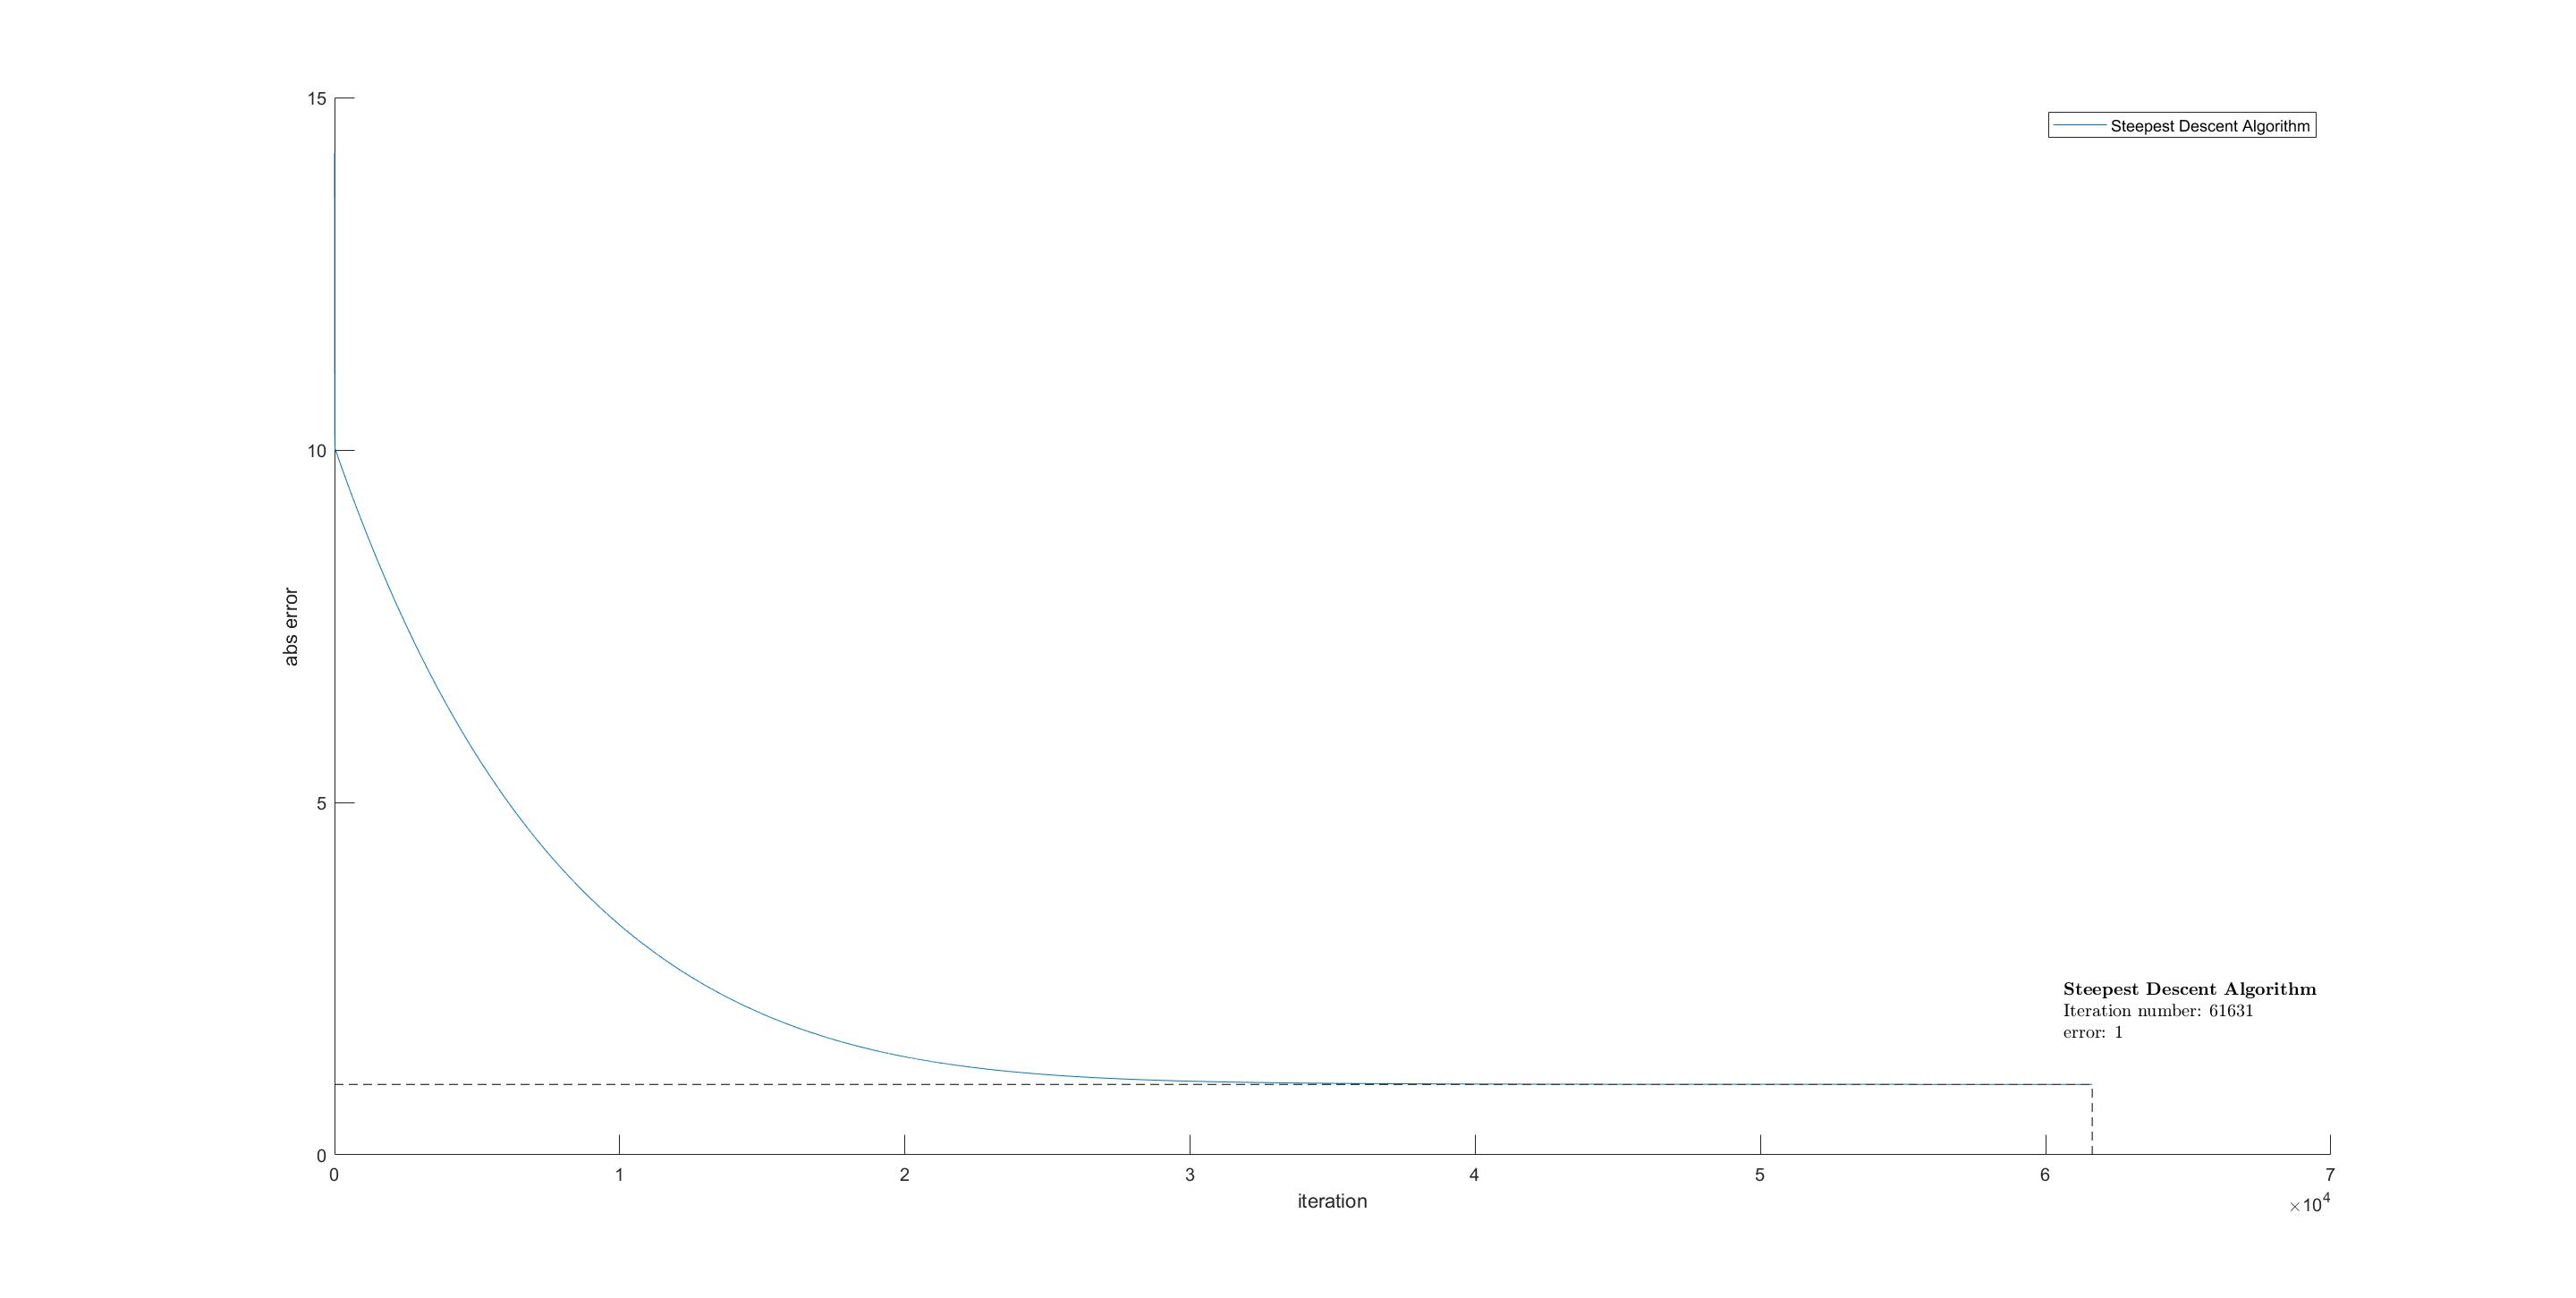
\includegraphics[width=\textwidth]{fig/IAvsSDA.jpg}
%	\caption{Steepest Descent Algorithm for Example \ref{ex:ILC:IAvsSDA}, with reference signal $r = (1 \; 1)^T$, $x_0 = 0$, $u_0 = 0$.}
%\end{figure}
%
%The algorithm converges and stops with error difference of $||e_{61631} - e_{61630}|| = 1.0178e-08$. 
%
%However, the error is not zero. Still, the numerical conditions does not allow to calculate a perfect solution, which is theoretically achievable. 





%In particular, let consider the scalar products 
%\begin{align}
%\langle y,z \rangle_m = \sum_{t = 0}^N y^T(t) Q(t) z(t)
%\end{align} 
%with $y(t), z(t) \in \R^m$ for $t = 1, 2, \dots, N$ and 
%\begin{align}
%\langle u,v \rangle_l = \sum_{t = 0}^N u^T(t) R(t) v(t)
%\end{align}
%with $u(t), v(t) \in \R^l$ for $t = 1, 2, \dots, N$.
%
%$Q(t) \in \R^{m\times m}$, $R(t)\in \R^{l\times l}$ for $0\leq t \leq N$ are here some positive definite weighting matrices. 
%
%The consideration from previous section do not change at all, if we set 


%
%
%
%With the choice of $Q(\cdot)$ we can
%\begin{enumerate}
%	\item emphasize some elements of inputs and outputs signals, depending on their importance in measuring accuracies and convergence rates,
%	\item emphasize the relative importance of different time intervals in measuring tracking accuracy and required convergence rates:
%	
%	for example, if we want to achieve a rapidly convergence in the initial parts of the time interval, we can set $Q(t) = \varepsilon^{2t}\tilde{Q}$ with some time independent $\tilde{Q}$ and $\varepsilon \in (0,1)$. 
%\end{enumerate}
%
%The choice of $R(\cdot)$ may arise out of real need to converge to a minimum input energy solution. 
%Again, using the $\varepsilon$-weighed $R(t) = \varepsilon^{2t}\tilde{R}$ with some fixed $\tilde{R}$, we can accent the input signals at some times $0\leq t_1 \leq t \leq t_2 \leq N$. This can be used if we want to limit the control action at some time intervals, or if we need to reflect the physical units used. 

\begin{exam}
	For the system \eqref{eq:ILC:Sys_ex1} we choose $N = 40$, $\beta = 0.0026$ and $R = I$, $Q = I$. The error evolution shows much more anticipated behavior (Figure \ref{img:ILC:SDA_N40}). The reference tracking is illustrated in Figure \ref{img:ILC:SDA_N40}. This time we have indeed the perfect following for the signal $r$. 
	
	\begin{figure}[ht]
		\centering
		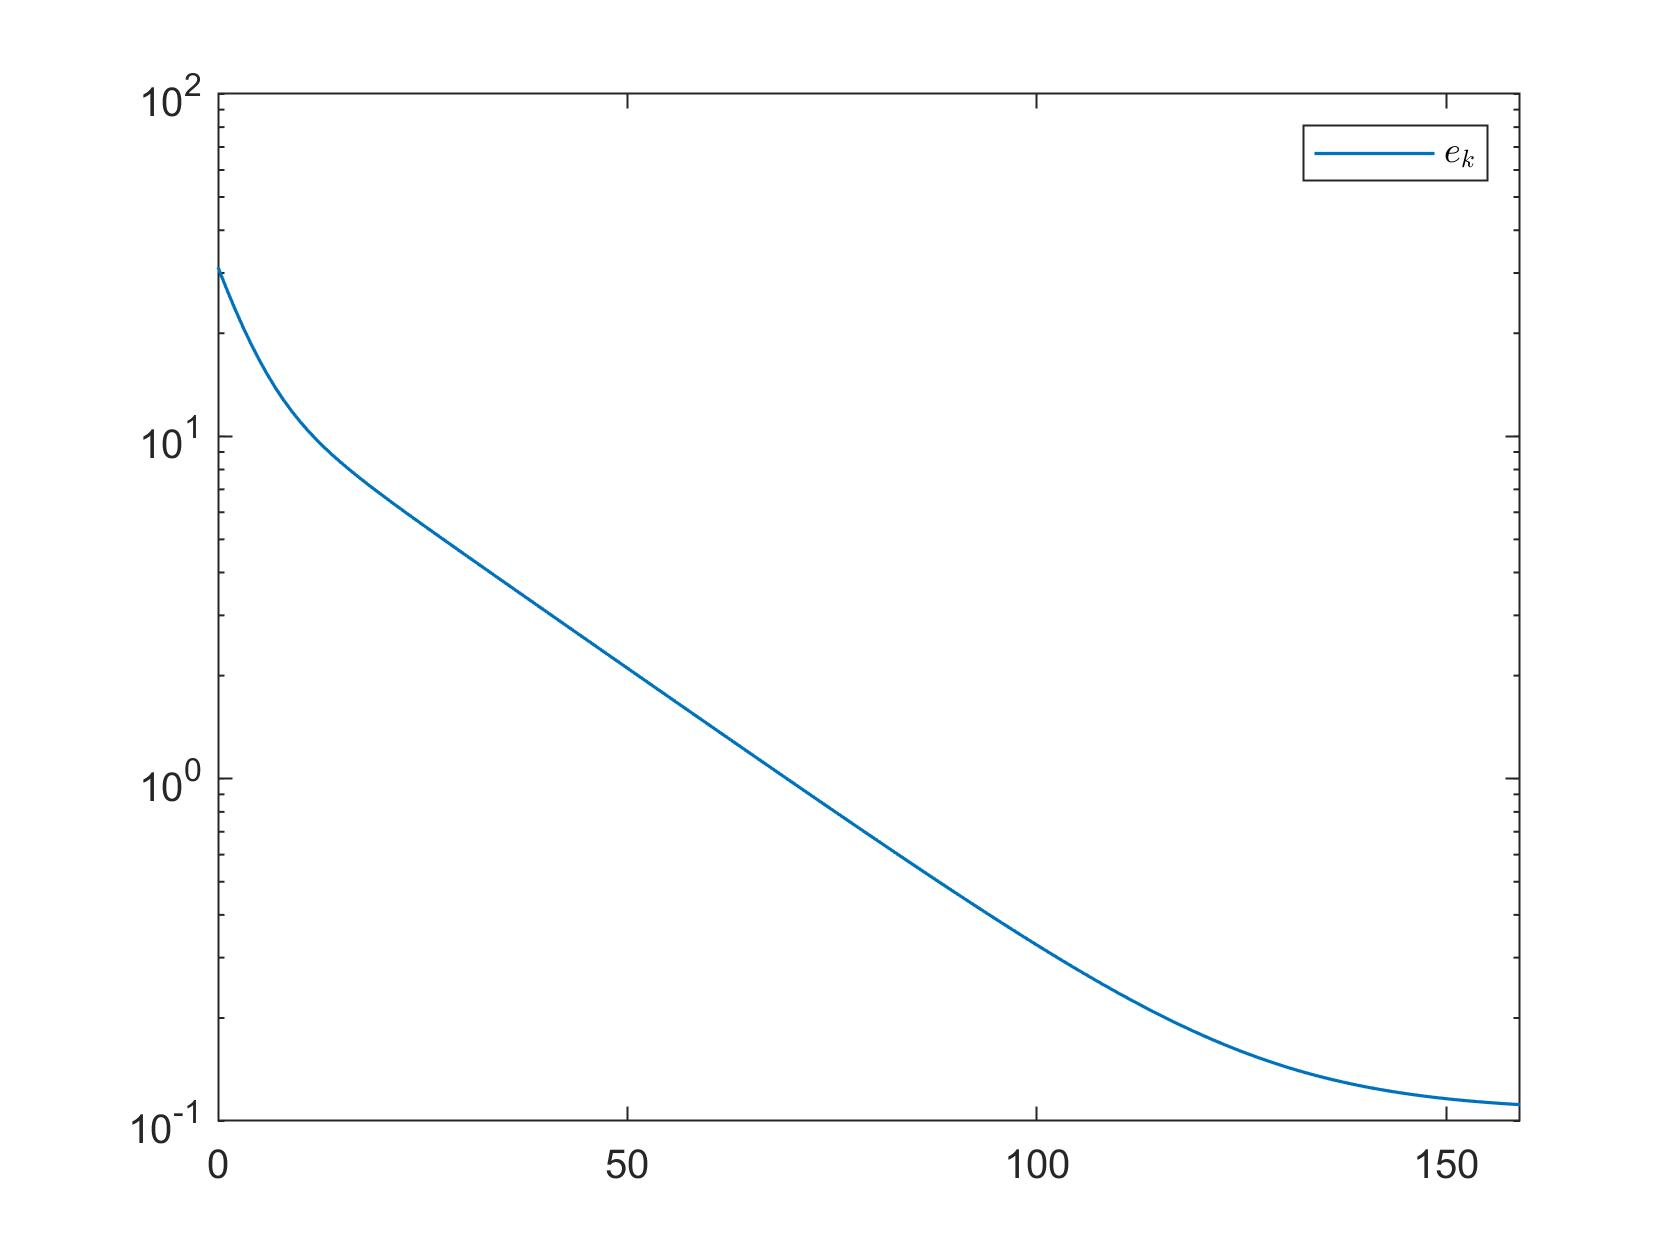
\includegraphics[width=\textwidth]{fig/SDA_N40.jpg}
		\caption{Error evolution with Steepest Descent Algorithm for the system \eqref{eq:ILC:Sys_ex1}}
		\label{img:ILC:SDA_N40}
	\end{figure}

	\begin{figure}[ht]
		\centering
	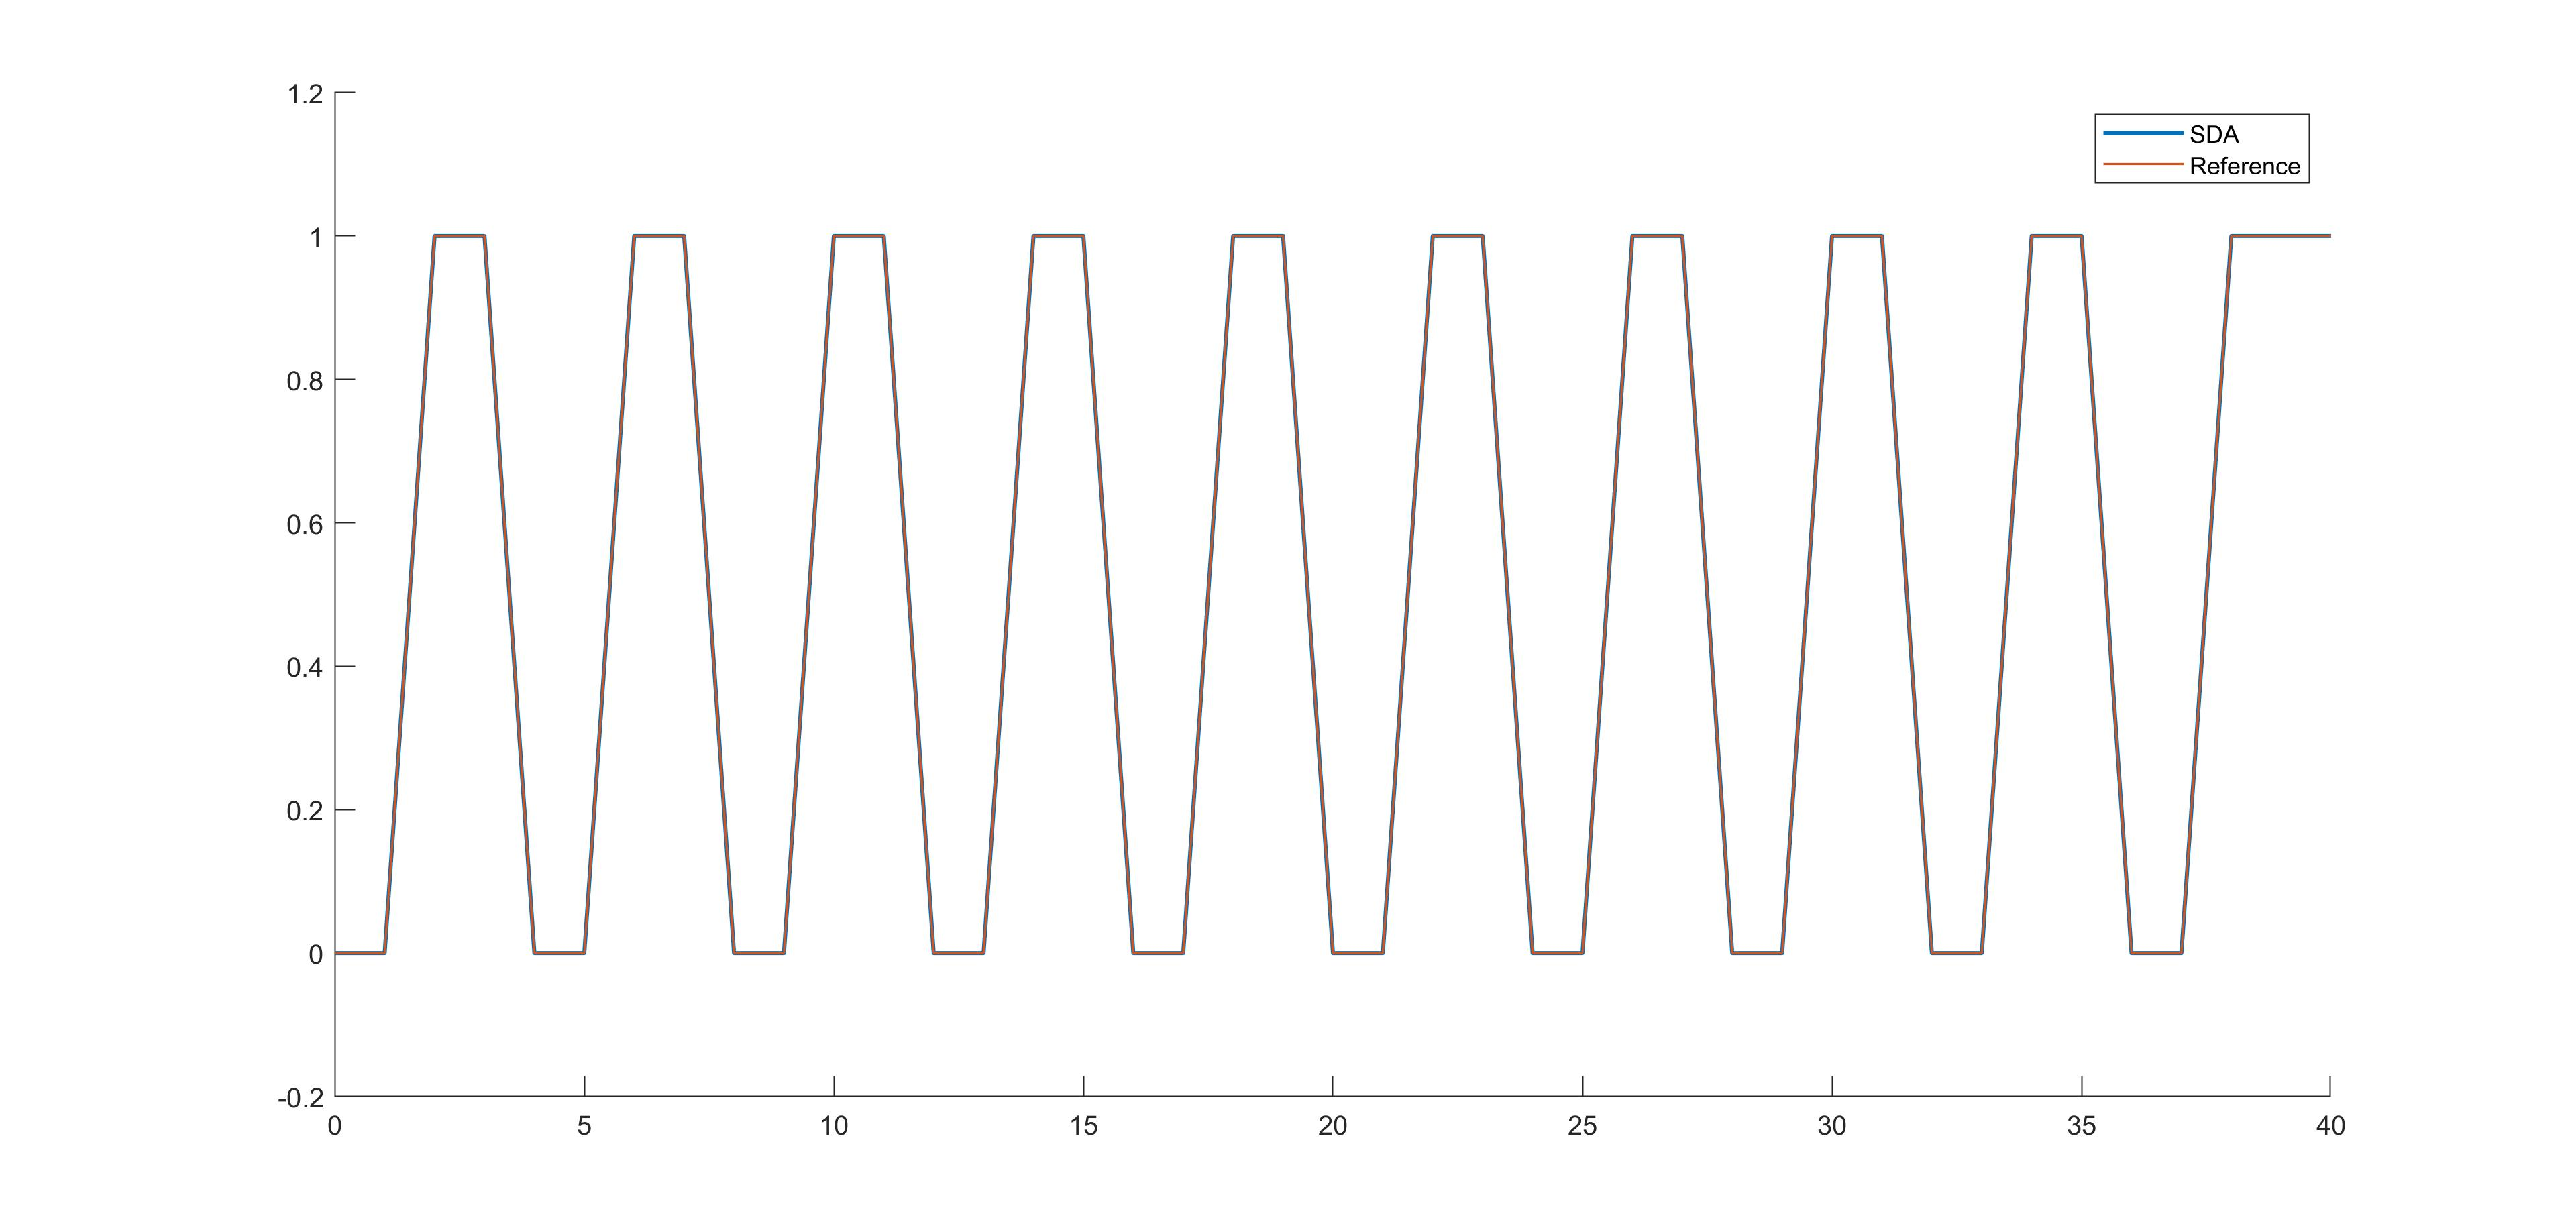
\includegraphics[width=\textwidth]{fig/SDA_N40_output.jpg}
	\caption{Reference signal tracking with Steepest Descent Algorithm for the system \eqref{eq:ILC:Sys_ex1}}
	\label{img:ILC:SDA_N40_output}
\end{figure}
\end{exam}


\subsection{Suppression of eigenvalues} 

In the considered algorithms we assumed the learning matrix $K$ to be constant for all iterations.
We can presume another controller structure and set variable $K_k$ for $k\geq 0$. 

The simplest modification way is to set an iteration varying gain $\beta$ for each step: $K_k = \beta_k K_0$, $k\geq 0$ ($K_0$ is here a fixed matrix).

Let us consider the eigenvalues of the matrix $GG^\star$ and choose the gains $\beta_k$, $k \geq 0$ according to them. 

\begin{theo}
	Assume, that the matrix $GG^\star$ has $q$ non-zero ordered eigenvalues $\lambda_0, \lambda_1, \dots ,  \lambda_q$. Set $\beta_k = \frac{1}{\lambda_k}$ for $k = 0, 1, \dots, \, q$ and consider the update law
	\begin{align}
	\label{eq:cl_var0}
	\begin{split}
	u_{k+1} &= u_k + \beta_k G^\star e_k, \\
	e _{k+1} &= (I - \beta_{k+1}  GG^\star) e_{k}  = \prod_{l = 0}^{k+1} (I - \beta_{l}  GG^\star) e_0, \; k\geq 0,\\
	u_0 &\in \R^{l (N+1)}.
	\end{split}
	\end{align}
	Then the error sequence $(e_k)_{k\geq 0}$ converges in a finite number of iterations.     
\end{theo}
\begin{proof} 
	Set $\t{N} := m(N+1) - 1$. With spectral theorem, there exists a basis of the eigenvectors $\{v_0, v_1, \dots, v_{\t N}\}$ with corresponding eigenvalues $\lambda_0, \lambda_1, \dots, \lambda_q, 0, \dots 0$. 
	Then we can write $e_0$ as 
	\begin{align}
	e_0 = \sum_{p = 0}^{\t N} \gamma_p v_p
	\end{align}
	for some uniquely defined $\gamma_p \in \R$, $p = 0, 1, \dots, \t N$. 
	
	For $k \in \N$ it follows 
	\begin{align}
	e_k = \left(\prod_{j=0}^k(I - \beta_j G G^\star)\right)e_0 = \sum_{p = 0}^{\t N} \gamma_p \left(\prod_{j=0}^k (I - \beta_j \lambda_p I)\right)v_p.
	\end{align}
	
	For the first iteration the error becomes 
	\begin{align}
	e_1 = \sum_{p = 0}^{\t N} \gamma_p ( I - \beta_1 \lambda_p I) v_p = \sum_{p=1}^{\t N } \gamma_p ( I - \beta_1 \lambda_p I) v_p.
	\end{align}
	
	The component $v_0$ is eliminated from the error.
	Assuming, that for $k \geq 1$ the first $k$ components are eliminated, we get 
	\begin{align}
	e_{k+1} = \sum_{p = 0}^{\t N} \gamma_p \left(\prod_{j=0}^k (I - \beta_j \lambda_p I)\right)v_p = \sum_{p = k + 1}^{\t N} \gamma_p \left(\prod_{j = 0}^k (I - \beta_j \lambda_p I )\right),
	\end{align}
	and hence the first $k+1$ components $v_0, v_1, \dots, v_k$ are eliminated. 
	By induction, the iteration process terminates after, at most,  $m(N+1) - q - 1$ iterations, as all non-zero eigenvalues have been covered and hence all corresponding eigenvectors are eliminated.	
\end{proof}

Although conceptually interesting this algorithm is not well applicable for the real problems. One can see, that the small non-zero eigenvalues of $GG^\star$ will lead to very large values of $\beta_k$ and hence we get extremely large transient variations in error norm. 
%The model errors can make this problem intolerable when elimination of eigenvector components will not be achieved in any iteration and/ or may be re-introduced in later iterations. 

Also computing the eigenvalues can be numerically questionable. Moreover, to achieve the monotonic convergence we need to consider only the eigenvalues $\lambda > \frac{1}{\sigma_{\max}^2}$.
If our model is inaccurate, and some eigenvalues are uncertain, it has directly impact on the iteration result. 

That all makes this algorithm not solid. Still, we can use the idea, to apply the eigenvalues of $G G^{\star}$ -- but not directly. We can try to ''pick'' the compatible eigenvalues.
\begin{alg}
	Choose a finite number $N_p + 1$ of points $p_0, p_1, \dots$ spread over the half-open interval $(\frac{1}{2}\sigma_{\max}^2, \sigma_{\max}^2]$. 
	The Gradient Algorithm with Suppression of Eigenvalues is defined via choosing of the iteration-depending control law  $K_k = \beta_k G^\star e_k$, where 
	\begin{align}
	\begin{split}
	\beta_k &= \frac{1}{p_k} \text{ for } k = 0 , 1, \dots , N_p,\\
	\beta_k &= \beta  \text{ for } k > N_p,
	\end{split}
	\end{align}
	with $\beta \in (0, \frac{2}{\sigma_{\max}^2})$.
	The iteration law is given via
	\begin{align}
	\begin{split}
	u_{k+1} &= u_k + \beta_k G^\star e_k, \; k\geq 0\\
	e _{k} &= \left[\prod_{l = 0}^k (I - \beta_l  GG^\star) \right] e_{0}, \;  k = 0 , 1, \dots , N_p,\\
	e _{k} &=  (I - \beta GG^\star)^{k - N_p} e_{N_p}, \;  k > N_p, \\
	e_0 &= r -  Gu_0 -d, \text{ } u_0 \in \R^{l (N+1)}.
	\end{split}
	\end{align}	
\end{alg}

This algorithm has the same convergence properties as Algorithm \ref{alg: SDA}, but potentially better convergence rates due to the eigenvalue suppression. Intuitively, the approach will increase the convergence speed in the first $N_p + 1$ iterations, if $N_p$ is large enough for good approximation of the interval $(\frac{1}{2} \sigma_{\max}^2, \sigma_{\max}^2]$.

\begin{exam}
	We apply the SoE Algorithm on the system \eqref{eq:ILC:Sys_ex1}. The error evolution we get is illustrated in Figure \ref{img:ILC:SDAvsSE}. The new algorithm needs only 148 iteration, while classical SDA terminates by 382 iterations. We also get a much better improvement $||e_0/e_\infty||$, while $e_\infty$  is meant to be the error in the last iteration. 
	
	In fact, for each eigenvalue $\lambda$ of $G G^\star$ holds 
	\begin{align}
	\lambda > 2/\sigma_{\max} = .1444. 
	\end{align}
	
	This explained the better performance of the algorithm, and better convergence rate.  		
	\begin{figure}[ht]
		\centering
		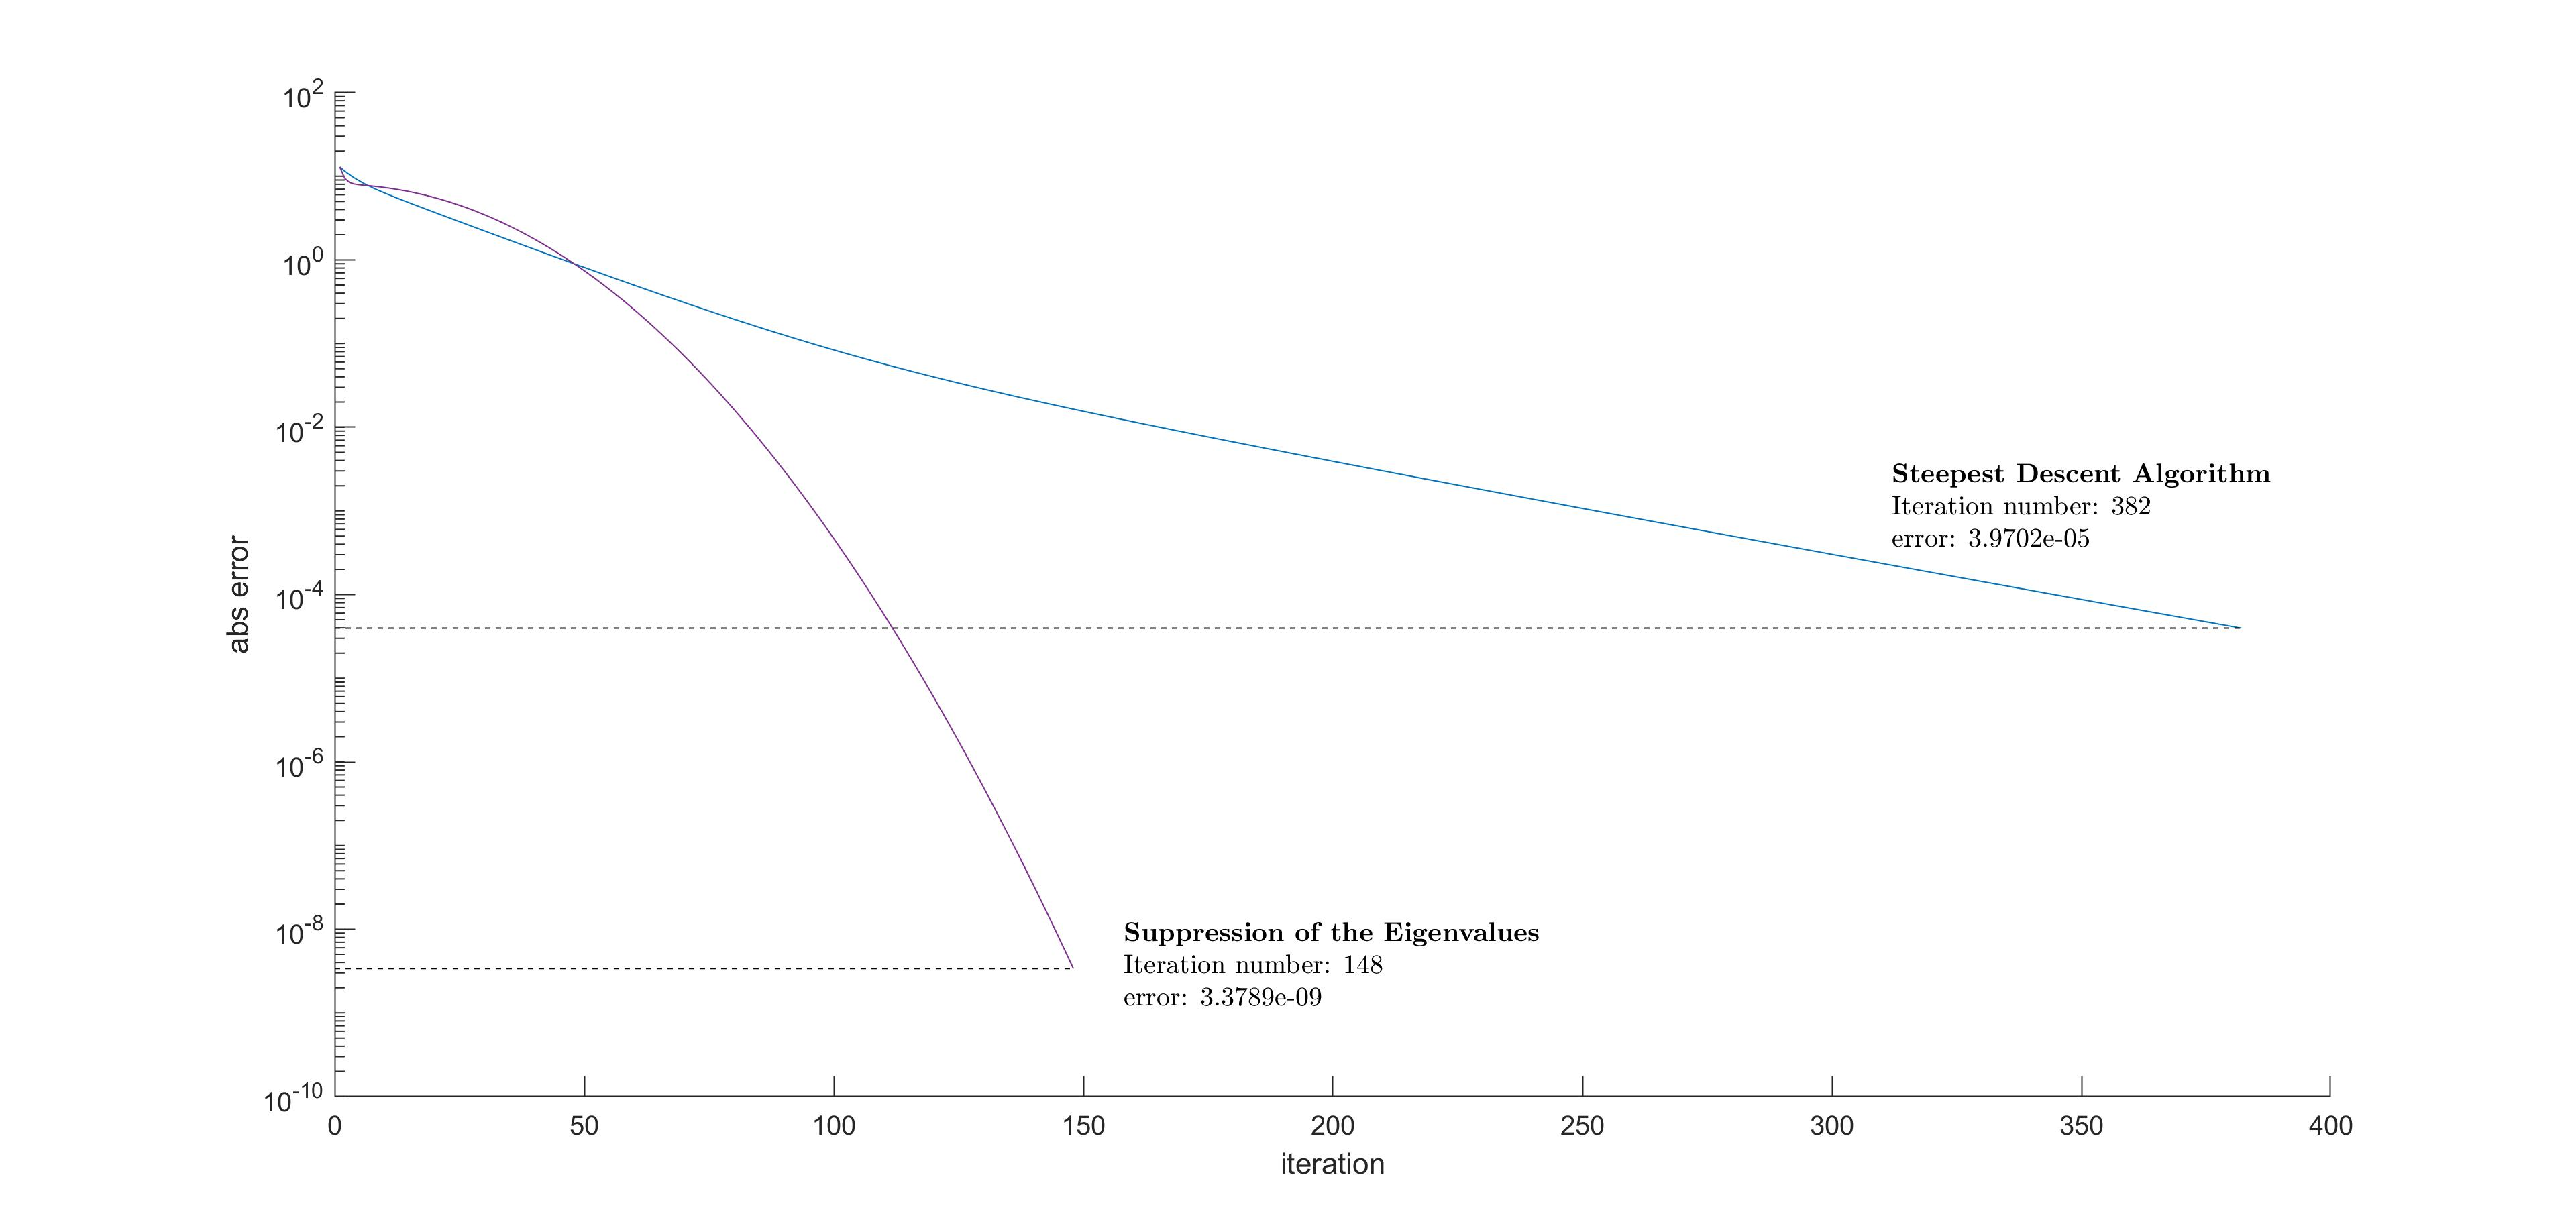
\includegraphics[width=\textwidth]{fig/SDAvsSE.jpg}
		\caption{Error evolution for classical SDA and SoE for system \eqref{eq:ILC:Sys_ex1}}
		\label{img:ILC:SDAvsSE}
	\end{figure}
	
\end{exam}

\section{Feedback Design}

With the previous algorithms we can achieve a better tracking for repetitively executed processes.  But they do not accent the special features of the model. For example, we can not manage the non-minimum-phase zeros, which can impact the convergence rate \cite{ILC}. 
If we consider the plant structure and construct a feedback controller, and then converts it into a steepest descent-like algorithm, we possibly can achieve better performance and robustness properties. 

More precisely, we consider a forward path compensator $K_c$ in a unity negative feedback system for \eqref{eq:GP}. 
The design criteria for $K_c$ include the closed-loop stability and the ability to track, albeit approximately, the reference signal $r$. With this compensator, depending on the model, we can remedy the plant properties such as oscillation, loop interaction, or the effects of non-minimum-phase zeros. 

We denote the closed-loop matrix $T$ and sensitivity matrix $S$ of the resultant closed-loop system by
\begin{align}
T = (I + G K_c)^{-1}G K_c \text{ and } S  = I - T =  (I + G K_c)^{-1}.
\end{align}

Then the compensated Steepest Descent Algorithm is given as follows. 

\begin{alg}
	\label{alg: FBDesign}
	The compensated Steepest Descent Algorithm is  is characterized by choosing  $K = \beta K_c S$, $\beta \in \R$. 
	The iterative law is given via 
	\begin{align}
	\label{eq:errFBDesign}
	\begin{split}
	u_{k+1} &= u_k + \beta K_c S T^* e_k, \\
	e_{k+1} &= (I- \beta T T^*) e_{k}, \; k\geq 0,\\
	u_0& \in \R^{l (N+1)}. 
	\end{split}	
	\end{align}
	Monotonic convergence to 
	\begin{align}
	\label{eq:FDErrLim} 
	e_\infty  = \lim_{k\to\infty} e_k = P_{\ker[T^*]}e_0,
	\end{align} 
	is guaranteed if
	\begin{align*}
	0 <\beta < \frac{2}{\sigma_{\max}(T)^2}.
\end{align*}
$T^*$ stays here for conjugate transpose of the matrix $T$. 
\end{alg}

One can see, that the error evolution corresponds to this of the model $y = T \tilde{u} + d$ with input $\tilde{u} 
\in \R^{m(N+1)}$, if we apply on it the Steepest Descent Algorithm.

The effect of the operator $T T^*$ can be seen by considering the closed-loop relation 
\begin{align}
y = Tr.
\end{align}
We get a perfect tracking, if $T = I$, which is not achievable by feedback control. Still, we can assume a good tracking if $||T|| \approx 1$. 

Therefore if $K_c$ provides excellent feedback control of $G$, then rapid convergence could be attained with a choice of gain $\beta \approx 1$. % if and the dominant frequency content of the reference $r$ lies in the bandwidth of the closed loop system $T$







